\chapter{Capzip simulations} \label{chapter:capzip_results}

In Chapter \ref{chapter:intro} we introduced the molecule capzip and its properties, highlighting the unknowns of its mechanisms of action. In Chapter \ref{chapter:MD} we presented a review on Molecular Dynamics simulations, proving their past successes in elucidating the behaviour of self-assembling and antimicrobial peptides.
%
Now, we employ this technique to understand better our system of interest. Given the exoticism of the unit, and the little atomistic information at disposal, modelling such peptide must proceed in a stepwise manner.

The first aim is to elucidate which structures it forms in solution and what interactions are keeping the molecules together. To understand the latter it is important to retain the highest level of detail possible, and for this reason we resorted to atomistic simulations first.
%
This description has an high computational cost though, preventing the simulation of very large systems for a very long time, as it would be required to reproduce the natural assembly from a dispersed solution.
%
Thus, we simulated increasingly complex pre-assembled blocks, verifying each time their behaviour in solution and inferring whether they are suitable to form a stable supramolecular structure. This approach, fully explained in Section \ref{sec:build}, lead to the model of a minimal capsule, which has been subsequently investigated at coarser levels to explore its behaviour on longer time scales.

This multiscale approach constitutes also an interesting methodological investigation as, to our knowledge, it compares for the first time the performances of the SIRAH force field \citep{Machado2018} versus the MARTINI \citep{Marrink2007, Monticelli2008} one, without or with polar water \citep{Yesylevskyy2010}. Indeed, when choosing a coarse grain representation, it is crucial to understand which aspects of the parametrisation are closer to its atomistic counterpart and which are instead more approximate. This helps in selecting the appropriate description for the system and the questions investigated.

Out of the pre-built capzip structures, a few selected ones were simulated in contact with model membranes, bacterial and mammalian, to understand the determinants of their antimicrobial activity. Details on these simulations and the specific techniques employed to promote the interaction are given in Section \ref{sec:details}.

\begin{figure}[p]
\centering
\subbottom[]{%
\includegraphics[width=0.9\linewidth]{3results_capsule/pics/merged_figures_beta_sheet} \label{fig:hb_beta_SIhere_hb}} \\
\bigskip
\subbottom[]{%
\includegraphics[width=0.47\linewidth]{3results_capsule/pics/pi_stacking_0} \label{fig:hb_beta_SIhere_pi1}} \hspace{0.2cm}
\subbottom[]{%
\includegraphics[width=0.47\linewidth]{3results_capsule/pics/pi_stacking_90} \label{fig:hb_beta_SIhere_pi2}}
\caption[Hydrogen bonds and $\pi$-stacking in a RRWTWE $\beta$-sheet]{(a) Presence of backbone hydrogen bonds between two facing antiparallel RRWTWE chains. The top right inset shows a scheme of the initial configuration. All the pairs highlighted in blue, green and pink are monitored and reported in the histogram (labels by amino acid pairs, named as in the inset figure and underlined with matching color); occupancy is averaged over 16 simulations of 20 ns. (b, c) For each replica and possible pair of facing Tryptophan residues in the $\beta$-sheet, the map gives the fraction of time for which a parallel or perpendicular $\pi$-stacking interaction has been observed. The second and third column correspond to pairs interacting by backbone hydrogen bonds.}
\label{fig:hb_beta_SIhere}
\end{figure}

\section{Modelling the assembly} \label{sec:build}

As previously mentioned, the antimicrobial sequence of capzip is designed with opposite charges at its extremes to favour an antiparallel $\beta$-sheets pairing with other copies of itself.
%
MD simulations of two RRWTWE sequences paired in this fashion confirm that the assembly is stabilised by the interactions between opposite charges (statistics gathered over 16 replicas, each run for 20 ns).
%
Moreover, backbone hydrogen bonds form between Tryptophan residues of facing strands, after a rearrangement of the mutual position of the residues which brings Trp ones in front of each other (Figure \ref{fig:hb_beta_SIhere_hb}).
%
Finally, $\pi$-stacking between Tryptophan side chains contributes to the interaction as well, albeit in minor measure (Figure \ref{fig:hb_beta_SIhere_pi1}, \subcaptionref{fig:hb_beta_SIhere_pi2}; details on its computation are explained in Section \ref{sec:analysis}).

Analogous simulations of two RRWTWE sequences paired in a parallel way show loosening of the pairing and in some cases the flip of one sequence to rearrange with respect to the other in the antiparallel manner, confirming that the antiparallel arrangement is favoured.

\begin{figure}[p!]
\centering
\subbottom[]{%
    \includegraphics[width=0.4\linewidth]{3results_capsule/pics/beta_trpHbonds} \label{fig:BTI_vmd_1} }
\hspace{0.05\linewidth}
\subbottom[]{%
	\includegraphics[width=0.4\linewidth]{3results_capsule/pics/beta_surf} \label{fig:BTI_vmd_1a}}
\subbottom[]{%
	\includegraphics[width=0.45\linewidth]{3results_capsule/pics/pentamer_restype.png} \label{fig:BTI_vmd_2}}
\subbottom[]{%
	\includegraphics[width=0.45\linewidth]{3results_capsule/pics/soccer_empos_extern_superimposed.png} \label{fig:BTI_vmd_3}}
\caption[Building blocks of capzip assembly]{(a) Detail of $\beta$-sheet pairing with facing Tryptophan residues forming hydrogen bonds between their backbone atoms (bonds representation coloured by residue type, hydrogen bond in dashes). (b) Two stacking $\beta$-sheets in surface representation, coloured by residue type. In white the partially buried hydrophobic surface. (c) A pentagonal subunit (bonds and cartoon representation): ten antimicrobial molecules arranged in two stacking pentagons. Capzip arms are paired in antiparallel $\beta$-sheets to form each pentagon, and the two are facing with their Tryptophan residues in contact. (d) Atomistic structure of the buckyball simulated (bonds and cartoon representation) and geometrical model for comparison. [VMD software \citet{HUMP96}]}
\label{fig:BTI_vmd}
\end{figure}
%PUT YELLOW-GREEN SCHEME COLOUR AS IN THE FOLLOWING + SUPERIMPOSE TRANSPARENT SURFACE TO SHOW RESIDUE TYPE

The hydrophobic interactions between Tryptophan residues (in white in Figure \ref{fig:BTI_vmd_1}) result in the creation of a hydrophobic patch which includes four of them on one side of the $\beta$-sheet plane.
%
This creates an amphiphilic structure where the hydrophobic core is segregated from the remaining charged residues distributed around.
%
The combination of two stacking $\beta$-sheets, paired to match their hydrophobic patches, constitutes an effective supramolecular assemblies to reduce the solvent exposure of such residues.

This pairing strategy, however, needs to be applied in the context of assembly of complete molecules.
%
The quasi three-fold symmetry of capzip suggests a regular geometric arrangement; even if simulations of a single molecule in solution highlight its flexibility, proposing that multiple arrangements can be accommodated by the molecule.
%
The best examples of geometrically organised protein structures can be found in viral capsids, which are composed by the regular repetition of highly symmetric protein subunits.
%
Inspired by this, we tested whether a geometrical organisation can represent a stable capsule, choosing as minimal representative geometry a truncated icosahedron (buckyball). This shape has 12 pentagonal faces and 20 hexagonal ones.

Preliminary atomistic simulations (100 ns) were run on a pentagonal subunit (Figure \ref{fig:BTI_vmd_2}), where ten antimicrobial molecules arranged in two stacking pentagons. Capzip arms are paired in antiparallel $\beta$-sheets to form each pentagon, and the two of them are facing with their Tryptophan residues in contact.
%
The simulations prove the cohesion between molecules belonging to the subunit. Specifically, the number of contacts between backbone $C_\alpha$s augmented slightly in the first 20 ns (Figure \ref{fig:penta_results_here_1}), due to the compaction of the unpaired external arms toward the core of the structure (see Figure \ref{fig:penta_results_SI} in SI Section \ref{sec:ch3_SI}).
%
Moreover, for each pair of facing chains (see definition in Figure \ref{fig:penta_results_here_2} legend), we computed the distance between their centres of mass. Figure \ref{fig:penta_results_here_2} reports the variance of these distances normalised by their average value, as a measure of the cohesion of the subunit, showing that in the majority of the cases less than 2\% of variability is observed. Overall, the block is not rigid, and does indeed deform and go back to the pentagonal shape multiple times in the simulations, but it is keeping the original pairing of the molecules.
% RUN SECOND SIMULATION?
\begin{figure}[t]
\centering
\subbottom[]{\includegraphics[width=0.48\linewidth]{3results_capsule/pics/bb_contacts.png} \label{fig:penta_results_here_1}}
\subbottom[]{\includegraphics[width=0.48\linewidth]{3results_capsule/pics/chain_COM_distance.png} \label{fig:penta_results_here_2}}
\caption[Cohesion measures on the pentagonal subunit]{(a) Number of backbone contacts during a simulation of a pentagonal subunit. (b) Variability of the inter chain average distance between the 30 facing chains in the pentagon. The 30 pairs defined as facing are the chains belonging to the same $\beta$-sheet (5 for each of the two stacking pentagons), and for each stacking $\beta$-sheet the 4 possible inter-pentagon (inter-layer) pairs of chains.}
\label{fig:penta_results_here}
\end{figure}

The pentagonal subunit respects the building principles of a) $\beta$-sheet pairing between antimicrobial sequences and b) double layer structure to screen the hydrophobic patches. Thus twelve of these units can be used to build a truncated icosahedron (Figure \ref{fig:BTI_vmd_3}), constituting its pentagonal faces (the hexagonal ones are formed by consequence by the branches extending from the pentagon).

Each capzip molecule is centred in one vertex of the polygon, with the branches laying alongside the edges departing from it. On each edge two branches coming from opposite sides meet in an antiparallel fashion. When possible, they are tightly paired in $\beta$-sheets with facing Tryptophan residues (as in Figure \ref{fig:BTI_vmd_1}). The stacking pentagons interact through the hydrophobic patches of their $\beta$-sheet, which are arranged in facing positions, with interdigitating Tryptophan if possible.
%
The full truncated icosahedron (Figure \ref{fig:BTI_vmd_3}) has two concentric layers, for a total of 120 molecules, and initial radius of 7.7 nm.
%
As anticipated, this geometry represents a minimal model of the possible structures capzip adopts in solution. Given the flexibility of the molecule, different arrangements are possible, though they are likely proceeding from analogous interactions between the minimal components (the arms of capzip).

The final structure was simulated at atomistic and coarse-grain levels, respectively with the GROMOS 53A6 \citep{Oostenbrink2004}, SIRAH \citep{Machado2018} and MARTINI \citep{Marrink2007, Monticelli2008} force fields (with both standard and polar water \citep{Yesylevskyy2010}).
% LEAVE?
From the final configurations of the MARTINI coarse-grain model (standard water), atomistic coordinates were obtained and simulated, to be compared with the original atomistic dynamics.
%
%Proving the stability at different timescales ascertains the characteristics that favour the assembly and identify the ones with suboptimal fitness to select them for improvement.
Moreover, additional simulations were run at all the coarse-grain levels on a structure made of one layer only (i.e.\ built from pentagonal subunits made by one pentagon only), to prove whether the bilayer is more energetically favoured.

Finally, a preliminary study on self-assembly was performed with one of the coarse grain representations (MARTINI with standard water), starting from capzip molecules randomly placed in solution.

A multiscale analysis is needed also to investigate the antimicrobial activity. Being highly costing to simulate a full truncated icosahedron on a bilayer patch at the atomistic level, the pentagonal subunit employed to build the complete structure (Figure \ref{fig:BTI_vmd_2}) was taken as representative of the latter. It was simulated close to the membrane plane, parallel to it, to avoid spending time in sampling conformations with the peptide far from the membrane (Figure \ref{fig:pL6_vmd_1}). This, together with a tailored use of an applied electric field (see Section \ref{sec:details}), speeds up simulations considerably.
%
To observe the natural binding of the peptide to the membrane, the process of the full buckyball approaching a model membrane was simulated with a MARTINI coarse-grain description (Figure \ref{fig:pL6_vmd_2}). The use of the MARTINI polar water \citep{Yesylevskyy2010} allowed the introduction of an external electric field, to compare the coarse grain simulations with the atomistic ones which employ analogous conditions.

% TRUE ONLY IF COMPLETED DPPC
Two membrane patches were simulated for both resolutions, a model bacterial and a model mammalian membrane, to identify the different interactions with the peptide. The first one presents 25\% of anionic lipids (DLPG), and the remaining zwitterionic (DLPC), while the second has only DLPC lipids. The choice of the bacterial model was dictated by the experiments performed on capzip \citep{Castelletto2016}, and the mammalian one was built with the same zwitterionic lipid as for the bacterial to simplify the comparison, e.g.\ to have membranes with comparable thickness and mechanical properties.

\begin{figure}[t]
\centering
\subbottom[]{\includegraphics[width=0.45\linewidth]{3results_capsule/pics/pL6_Pramp_pic2.png} \label{fig:pL6_vmd_1}}
\subbottom[]{\includegraphics[width=0.45\linewidth]{3results_capsule/pics/fig7_irene.png} \label{fig:pL6_vmd_2}}
\caption[Snapshot of simulations of capzip on model membranes]{(a) Atomistic structure of a pentagonal subunit on a 740 lipid bacterial model membrane of composition DLPC:DLPG 3:1 (initial configuration). Peptide backbone in line and cartoon representation; lipid in cyan lines (DLPC) and blue ones (DLPC), all lipids phosphate in golden van der Waals beads. (b) coarse-grain (MARTINI) representation of the buckyball on a 2880 lipids bacterial model membrane (final configuration of the trajectory). Protein in bonds representation: green outer buckyball layer, yellow inner one. Lipid in line representation, coloured by bead type, and lipids phosphate in golden van der Waals beads. [VMD software \citet{HUMP96}]}
\label{fig:pL6_vmd}
\end{figure}
\section{Simulations details} \label{sec:details}

All simulations were performed with the GROMACS software, version 5.5 and 2016 \citep{Berendsen1995,Abraham2015,gromacs_man}. 

\subsection{Atomistic simulations}
\paragraph{Simulations in solution} The atomistic coordinates for the peptidic supramolecular assemblies described in Section \ref{sec:build} (Figure \ref{fig:BTI_vmd_3}) were built combining GROMACS tools and the MOE software \citep{moe}.
%
Simulations were run with the GROMOS 53A6 force field \citep{Oostenbrink2004}. Parameters for the central residue connected with the peptidic chains were computed with the ATB software \citep{Malde2011, Koziara2014}; the ones for the bonds joining this residue to the antimicrobial side chains were derived from the values tabulated in the force field for analogous ones.
%
A python module has been designed to manipulate GROMACS topology objects for the GROMOS force field and add peptide bonds at the location required (see Appendix \ref{sec:Appendix_software} for details). This is useful for multibranched peptides which are not supported by the standard GROMACS tools, and for which a manual implementation would be otherwise needed.

The systems were solvated with single point charge (SPC) water \citep{Berendsen1981} and counter ions were added (Na$^+$ or Cl$^-$); further ions were introduced to reach the concentration of 150 mM, to reproduce the experimental conditions. Given the presence of counter ions, the species to which they belong had a slightly higher concentration.
%
For simulations of a single $\beta$-sheets and of the pentagonal subunit, the systems were energy minimised with a steepest descent algorithm, then equilibrated in the NVT ensemble with decreasing positional restraints at increasing temperatures (100 K, 200 K, 250 K, 300 K and respectively 1000, 1000, 500, 250 kJ/mol$\cdot$nm$^2$ restraints, 100 ps each); then in the NPT ensemble, without restraints, at the same temperatures steps and for the same time. Production followed for 100 ns.

For the truncated icosahedron structure the above equilibration was insufficient. Due to the construction procedure, two thirds of the branches are not properly paired along the edges.
%
Therefore, after an NVT equilibration as above, strong flat-bottom restrains (1000 kJ/mol$\cdot$nm$^2$) were placed between the center of mass of imperfectly aligned branches throughout the NPT heating, to penalise their mutual separation with respect to their initial distance (100 ps runs at 100 K, 200 K and 250 K and 35 ns at 300 K).
%
This was followed by a series of 10 ns runs at 300 K with decreasing flat-bottom restraints strength (750, 500 and 250 kJ/mol$\cdot$nm$^2$) and by a free production run (100 ns).
%
Three different replicas were run, generated from the final configuration of the 300 K NPT run with 1000 kJ/mol$\cdot$nm$^2$ restraints.

Throughout all the simulations, the temperature was maintained by independently coupling the protein and the solvent (plus ions) to two external temperature baths using a velocity rescale thermostat \citep{Bussi2007} with coupling constant $\tau _T$ of 0.1 ps. The pressure was kept at 1 bar by Berendsen \citep{Berendsen1984} or Parrinello-Rahman barostat \citep{Parrinello1981} (for the equilibration phases and the production run respectively) using an isotropic coupling, with isothermal compressibility of 4.5 $\times$ 10$^{-5}$ bar$^{-1}$ and coupling constant $\tau_P$ of 1 ps. Electrostatic interactions were treated using the smooth Particle Mesh Ewald (PME) algorithm \citep{Essmann1995}, with a short-range cutoff of 0.9 nm. The van der Waals interactions were treated with a plain 0.9 nm cutoff. All atomistic runs were performed using a 2 fs time step. An overview of the simulations of peptide assemblies in solution is given in Table \ref{table:sim_solution}.

\begin{figure}[t]
\centering
 \def\arraystretch{1.6}
\begin{tabular}{l|ccc}
 \multicolumn{4}{c}{\textbf{Capzip in solution simulations}} \\
 \hline
 System (Nr peptides) & FF & Time (ns) & Replicas \\
 \hline
 $\beta$-sheet (Fraction) & GR & 20 & 16 \\
 Pentagonal subunit (10) & GR & 100 & 1 \\
 Buckyball bilayer (120) & GR & 100 & 3 \\
 Bucky. bi (120) \& mono (60) & SI & 1000 & 3 \& 2 \\
 Bucky. bi (120) \& mono (60) & MA & 1000 & 3 \& 2 \\
 Bucky. bi (120) \& mono (60) & MA\_P & 1000 & 2 \& 2 \\
 Backmapped bucky. (120) & GR & 200 & 2 \\
 Random (60, 120, 480) & MA & 10000 & 1 \\
 \hline
 \end{tabular}
\captionof{table}[Simulations of capzip assemblies in water]{Table of simulations of capzip assembly in water. \emph{Bucky.\ bi} = buckyball bilayer; \emph{Bucky.\ mono} = buckyball monolayer. \emph{Random} = random configuration of capzip molecules in a box (see Section \ref{sec:MARTINI_sim_det}). Force field (FF): GR = united atom GROMOS 53A6 \citep{Oostenbrink2004}, SI = coarse-grain SIRAH \citep{Machado2018}, MA = coarse-grain MARTINI \citep{Marrink2007, Monticelli2008}, MA\_P = coarse-grain MARTINI with polar water \citep{Yesylevskyy2010}.}
\label{table:sim_solution}
\end{figure}

\paragraph{Simulation with membranes} The atomistic coordinates for the bacterial membrane patch were built with the PACKMOL software \citep{Martinez2009}, from pdb files of a single DLPC \citep{PogerOrig} and DLPG \citep{Kukol2009} molecule. Two patches were built, made respectively of 512 and 740 lipids, with composition DLPC:DLPG (3:1). The initial area per lipid was set to 0.70 nm$^2$, above the values found experimentally for either lipid species (0.608(12) nm$^2$ for DLPC \citep{Kucerka2011} and 0.656(12) nm$^2$ for DLPG \citep{Pan2012}). The correct area per lipid of the mixture was reached during a 400 ns equilibration (see details below), the final configuration of which was used for simulations with the peptide.
% VERIFY WE CAN RUN IT!!!
Given the analysis performed on the bacterial patch (see Section \ref{sec:lip_atom_bact}), for DLPC we opted for simulating a large membrane only. Accordingly, we produced a patch with 748 lipids and initial area per lipid of 0.68 nm$^2$.

For membrane-peptide atomistic simulations, the initial configuration was generated from the equilibrated bilayer and the equilibrated pentagonal subunit (after 100 ns run with positional restraints on the C$_\alpha$), placing the subunit plane parallel to the membrane and close to it (Figure \ref{fig:pL6_vmd}).
%
The inflategro script \citep{Kandt2007} was used to solve the partial overlap of peptide side chains with lipid molecules, removing the overlapping lipids if necessary.
%In the configuration chosen, 6 and 3 lipids are removed from the 512 and 740 lipids bacteria membrane patch respectively and 13 from the 748 mammalian membrane one.
%
The sizes of the two patches fit the pentagonal subunit with respectively 3.5 nm and 5.4 nm distance between its periodic boundary images (along both $x$ and $y$).

For simulations involving membranes, the version 54A7 of the GROMOS force field \citep{Schmid2011} was initially chosen and it is thus used for simulations of the 512 lipids patches, but upon further research version 54A8 \citep{Oostenbrink2005, Reif2013} was deemed more suitable ad thus selected for the runs on the larger patches. Lipid parameters were taken from \citep{PogerOrig} for DLPC, while for DLPG they were built from the ones available in the literature for POPG \citep{Kukol2009}.

The simulations set-up is as above, except for the use of three thermal coupling groups (peptide, membrane, water plus ions), a semi-isotropic pressure coupling, and a larger cut off radius for both Coulomb and van der Waals interactions (1.2 nm). Additionally, for the 512 lipids membrane, a Reaction Field \citep{Tironi1995} was used instead of PME long range electrostatic treatment (with cut off radius 1.4 nm). Control simulations on membrane patches without peptide showed that the results in terms of area per lipid are compatible with the ones obtained using PME.

Each membrane patch was first equilibrated for 50 ps in NPT conditions at 50 K, then the temperature was gradually increased up to 300 K in 500 ps, and finally a 400 ns production was run. A similar equilibration procedure was followed for peptide-membrane systems.

Additional simulations were performed applying an external electric field to the membrane, pointing from the side hosting the peptide to the opposite one, to mimic the membrane potential and verify how the peptide affects the response to external stimuli.
%
In a first run the field was increased by 20 mV/nm steps every 200 ns (or 10 mV/ns when reaching the critical value), until poration was induced (at 130 mV/nm).
%
Another simulation was performed for both the 512 and 740 lipids patches, with the threshold field, starting from the unperturbed membrane configuration (three replicas each).
%
As a control, analogous test simulations were run on the 512 lipids bacterial patch, assessing the electroporation threshold at the higher value of 140 mV/nm.

To be noticed that the field across the bacterial inner membrane can be estimated around 35 mV/nm, and across the mammalian one 20 mV/nm (from, respectively, a -130/-150 mV and -70/-90 mV potential \citep{Yeaman2003,Wilson2011} and an estimate membrane thickness of 4 nm). However, previous computational work often explored the effects of higher fields, up to 500 mV/nm \citep{Tieleman2004, Bockmann2008, Piggot2011}, to witness poration within the simulations time, according to the resources available.

An overview of the simulations of peptide-membrane systems is given in Table \ref{table:sim_membr} (control simulations on pure membrane are listed in SI Table \ref{table:SI_membrane}).
%
\begin{figure}[t!]
\centering
\vspace{3cm}
 \def\arraystretch{1.6}
\begin{tabular}{lccccc}
\multicolumn{6}{c}{\textbf{Capzip on membrane simulations}} \\
\hline
 & Peptides & Lipids &  $\,$Model$\,$ & Time ($\mu$s) & Replicas\\
 \hline
 \multirow{4}{*}{\rotatebox{90}{Bacterial}} & 10 & 512 & GR & 500 & 2 \\
 & 10 & 740 & GR & 500 & 1 \\
 & 120 & 2880 & MA & 10000 & 2 \\
 & 120 & 2880 & MA\_P & 10000 & 1 \\
 \hline
 \multirow{3}{*}{\rotatebox{90}{Mammalian}} & 10 & 740 & GR & 500 & 1 \\
 & 120 & 2880 & MA & 10000 & 1 \\
 & 120 & 2880 & MA\_P & 10000 & 1 \\
 \end{tabular}
 \begin{tabular}{lcccccc}
 \hline
 \multicolumn{7}{c}{\textbf{Capip on membrane \& electric field sim.}} \\
  \hline
  & Peptides & Lipids & $\,$Model$\,$ & $\,$Time (ns)$\,$ & E (mV/nm) & Rep. \\
 \hline
 \multirow{4}{*}{\rotatebox{90}{Bacterial}} & 10 & 512 & GR & 75$^P$, 20$^P$, 71$^P$ & 130 & 3 \\
 & 10 & 740 & GR & 60$^P$, 50$^P$, 70$^P$ & 130 & 3 \\
 %\hline
 & 120 & 2880 & MA\_P & 500 & 20 & 1 \\
 & 120 & 2880 & MA\_P & 168$^P$ & 40 & 1 \\
 \hline
 \multirow{3}{*}{\rotatebox{90}{Mamm.}} & 10 & 740 & GR & 20$^P$, 28$^P$, 39$^P$ & 130 & 3 \\
 & 10 & 2888 & MA\_P & 500 & 20 & 1 \\
 & 10 & 2888 & MA\_P & 500 & 40 & 1 \\
 \hline
\end{tabular}
\captionof{table}[Simulations of capzip assembly on membranes]{Table of simulations of peptide-membrane complexes. A number of 10 peptides denotes the pentagonal subunit, 120 the buckyball bilayer. Force fields (FF): GR = united atom GROMOS, MA = coarse-grain MARTINI, MA\_P = coarse-grain MARTINI with polar water. Superscript P denotes poration. For electroporation simulations on pure membranes, see SI Table \ref{table:SI_membrane}.}
\label{table:sim_membr}
\vspace{3cm}
\end{figure}

\subsection{SIRAH coarse-grain simulations}
SIRAH coarse-grain simulations were run with the SIRAH force field \citep{Machado2018}. Peptide coordinates for the buckyball geometry were obtained from the atomistic ones using the converter distributed with force field. Parameters for the central residue were built from comparison with similar chemical moieties. All simulations were run adding Cl$^-$ counter ions to balance the positive charges of the peptide and additional Na$^+$  and Cl$^-$ ones to reach a 150 mM concentration (of Na$^+$, slightly higher for Cl$^-$).

While for simulations of the peptide buckyball in solution our multiscale procedure includes SIRAH, for simulations on membranes we focussed on atomistic and MARTINI simulations only. This has been performed in the interest of time, and due to technical difficulties in preliminary SIRAH runs with membranes (in particular in tuning the pressure coupling).
%
This is likely due to a suboptimal equilibration procedure; indeed, there are few benchmarks on SIRAH for lipids so far \citep{Barrera2019}, and none for systems as large as the one studied here. We are continuing to explore the system, collaborating with the developers of the force field to work out the best equilibration procedure to treat large membrane patches.

For SIRAH simulations, the temperature coupling was performed with a velocity rescale thermostat \citep{Bussi2007} and coupling constant $\tau _T$ of 0.1 ps, and the pressure coupling at 1 bar pressure, with 4.5 $\times$ 10$^{-5}$ bar$^{-1}$ isothermal compressibility, using a Parrinello-Rahman barostat \citep{Parrinello1981} with a $\tau _P$ of 6 ps. Electrostatic interactions were treated using the PME algorithm \citep{Essmann1995}, with a short-range cutoff of 1.2 nm and relative dielectric constant of 1. The van der Waals interactions are treated with a plain 1.2 nm cutoff.

After energy minimization, a 4 ns NVT equilibration was run at 300 K, followed by a 10 ns NPT run, both with positional restraints (1000 kJ/mol$\cdot$nm$^2$) on the solute. Two 10 ns run (NPT ensemble, 300 K) were then performed with backbone restraints of 1000 and 100 kJ/mol$\cdot$nm$^2$, respectively. Similar to the procedure adopted for atomistic simulations, flat bottom positional restraints (1000 kJ/mol$\cdot$nm$^2$) were enforced on the unpaired branches during the latter. After this, three additional 10 ns equilibrations were run at 300 K, with no backbone restraints and decreasing flat bottom ones (respectively 750, 500 and 250 kJ/mol$\cdot$nm$^2$). Finally the production run was carried on for 1 $\mu$s. All runs were performed with a 20 fs time step.

\subsection{MARTINI coarse-grain simulations} \label{sec:MARTINI_sim_det}
For MARTINI \citep{Marrink2007, Monticelli2008} coarse-grain simulations, peptide coordinates were obtained from the atomistic ones using martinize.py \citep{DeJong2013} with a customised mapping for the central residue. Parameters were obtained with the same script for the arms, while pycgtool.py \citep{Graham2017} was used for the central residue. Parameters for the joining bonds were derived from tabulated values of analogous ones.

Initial coordinates for the self-assembly simulations were obtained with GROMACS tools, placing the desired amount of coarse grained molecules in the simulation box with random positions.
%
The side of the cubic box was chosen as 44 nm, and three different peptide concentrations were simulated: 1.25 mM (60 molecules), 2.50 mM (120 molecules) and 10 mM (480 molecules), all for 10 $\mu$s.

The bacterial and mammalian model membranes, hosting 2880 lipids each, were built with insane.py \citep{Wassenaar2015}, with composition DLPC:DLPG (3:1) and pure DLPC respectively. The simulations parameters used for lipids are consistent with \citet{SiewertJ.Marrink2003}. The peptide-membrane systems were built placing the buckyball at a minimum distance of 1 nm from the membrane surface.

For all standard MARTINI simulations, counter ions only were added, while for the ones run with Polar MARTINI, additional Na$^+$ and Cl$^-$ were inserted to reach a 150 mM concentration.

For simulations with the standard water model, the temperature coupling was performed with a velocity rescale thermostat \citep{Bussi2007} with a coupling constant $\tau _T$ of 1 ps. An isotropic or semi-isotropic pressure coupling was applied (simulations of peptide in solution and peptide on membrane respectively) at 1 bar pressure, with 4.6 $\times$ 10$^{-5}$ bar$^{-1}$ isothermal compressibility, using a Berendsen \citep{Berendsen1984} or Parrinello-Rahman barostat \citep{Parrinello1981} (equilibration and production phase respectively) with $\tau _P$ of 2 ps and 12 ps. An isotropic or semi-isotropic coupling has been used for simulation without and with membranes respectively.
%
Coulomb interactions were treated with a Reaction Field scheme \citep{Tironi1995} and cut off radius of 1.1 nm, van der Waals interaction with a cut off scheme and the same cut off radius. The relative dielectric constant is set to 15.
%
Simulations performed with the polar water model were run with the parameters above, except the relative dielectric constant set to 2.5, and the choice of a PME scheme for the long range Coulomb interaction (1.2 nm cut off radius).

For simulations of the capsule in solution, for both water models, after energy minimization, four 10 ns equilibration runs (NPT ensemble, 300 K, 10 fs time step) were performed with flat bottom positional restraints on the unpaired branches (respectively at 1000, 750, 500 and 250 kJ/mol$\cdot$nm$^2$) - as done for the other force fields.
%
Finally the production run was carried on for 1 $\mu$s. All runs were performed with a 20 fs time step.

It is interesting to notice that the MARTINI force field with the standard water model produced very similar results with or without such refined equilibration procedure, as confirmed by simulations of the buckyball run after a short unrestrained equilibration only (500 ps, 1 fs timestep). However, we choose to follow the same procedure as for the other force fields to have more consistent results, and be certain that the differences observed are due only to the parametrisation an not to the equilibration procedure.

From the final configurations of two out of the three standard MARTINI replicas, atomistic coordinates were obtained using the MARTINI backward tool (version 5) \citep{Wassenaar2014} and run for additional 200 ns with the set up used for atomistic simulations.

The equilibration for the self-assembly simulations (run only with the standard MARTINI model) included only an energy minimization, followed by a 1 ns equilibration with the Berendsen barostat, before switching to Parrinello-Rahman for the 10 $\mu$s production.

The membranes used in MARTINI simulations are equilibrated for 1 $\mu$s with standard water and the final configuration is used to build the peptide-membrane systems, together with the capsule structure (obtained after the equilibration runs). The full system is energy minimised, equilibrated for 500 ps and production is followed for 10 $\mu$s for simulations with the standard water, and 1 $\mu$s with polar water.

The adoption of polar water allows to perform electroporation experiments also with the MARTINI force field (while the standard water, not bearing a dipole, is unable to screen the externally applied electric field, resulting in unphysical effects).
%
We thus resorted to a procedure similar to the one employed for atomistic simulations, testing an external electric field of magnitude 20 mV/nm and 40 mV/nm, without proceeding further as the latter gave poration in presence of the peptide.
%
It is possible that longer simulations would allow to observe this behaviour even with lower values of the force field, however, in the interest of time, we selected these two values for further investigation.

We selected a configuration from the early stages of poration (at 40 mV/nm), where the pore showed a diameter of 2 nm, and prolonged the simulation switching to isotropic pressure coupling. This allows the pore to expand in a controlled manner. Indeed, in a semi-isotropic pressure coupling scenario, the pressure in the $z$ direction suddenly decreases when a pore forms (as water can pass through the membrane). The barostat algorithm reacts decreasing the $z$ side of the box, in an effort to restore the target pressure in this direction, but to accommodate all the molecules the box must necessarily expand in the $x$ and $y$ directions.

Control simulations with the two values of the electric field mentioned were performed on the membrane alone. The same procedure, i.e.\ simulations with capsule and electric field plus control simulations on the membrane only was applied to the pure DLPC membrane as well (save the additional simulation after poration, as this is not observed for this system).


\section{Analysis} \label{sec:analysis}

In Section \ref{sec:build} we presented an evaluation of the occurrence of $\pi$-stacking between Tryptophan residues in the $\beta$-sheet simulations. The computation was performed as follow: for each pair of Trp residues, we computed the minimum distance between the benzene ring of their side chain (in function of time), as well as the angle formed by their two planes. We defined a parallel $\pi$-stacking if the minimum distance was below 0.6 nm and the angle smaller than 45$^{\circ}$, while a perpendicular one if the minimum distance was below 0.6 nm and the angle between 75$^{\circ}$ and 105$^{\circ}$. Occupancy was found normalising the number of frames in which the interaction appeared by the number of frames considered for the analysis.    
    
\subsection{Simulations in solution}
Several analysis on the structure and chemico-physical properties of the buckyball in solution were performed on the outcome of the simulations.

\begin{itemize}
\item Radius of gyration ($R_g$), and Root Mean Square Deviation with respect to the initial configuration (RMSD) were computed (GROMACS).

\item To get the average distribution of the mass of the capsule around its center, the Radial Distribution Function (RDF) of protein masses around their center of mass was computed (GROMACS). The profile was fitted with a Gaussian function (R software \citep{R}): the position of its maximum can be taken as the average radius of the capsule, and its Full Width at Half Maximum (FWHM) as an estimate of the capsule wall thickness.

\item The dynamical character of the structure was assessed computing the correlation of motion between the molecules. The central atom (or bead) from which the branches depart was taken as reference. For all the pairs ($i, \, j$) of such reference positions, the covariance of motion was computed along each direction (GROMACS). The total covariance was obtained as: $\sigma^2(i,j) = \sigma_x^2(i,j) + \sigma_y^2(i,j) + \sigma_z^2(i,j)$. Finally the measure was normalised to obtain the correlation:
\begin{equation}
corr(i,j) = \frac{\sigma^2(i,j)}{\sqrt{\sigma^2(i,i)\,\cdot\,\sigma^2(j,j)}}.
\end{equation}

\item The pairing of the branches was quantified as follow. Two branches are defined as paired if their center of mass is closer than a cut off distance of 1.2 nm. This simple measure discards more precise information on the orientation of the chains with respect to each other, and aims at checking whether the network of molecules present in an ideal buckyball structure is maintained. In the ideal buckyball, contacts within the same layer sum up to 90 for each layer (180 in a bilayer). This measure can be easily applied to any description (atomistic or coarse-grain) without disagreement in the interpretation. Given the loose character of the measure, we considered only the pairings surviving more than 90\% of the simulation time.

\item To characterise the chemical determinants that promote the assembly, we investigated the interactions between amino acids of different types, computing the number of contacts between backbone and side chains of single amino acids, filtering for the ones present a least 50\% of the simulation time, and classifying them by amino acid type.
%
We define a contact between amino acids backbones if the C$\alpha$ of two residues (or the corresponding coarse-grain bead) are closer than a cutoff distance of 0.6 nm; and between side chains if selected reference atoms in the side chain are closer than the same cut off; finally mixed ones if the proximity is between a C$\alpha$ and the side chain reference atom. As side chains reference, we took the heavy atom or bead farthest away from the backbone (respectively for GROMOS, SIRAH and MARTINI: CZ/SC2/BCZ for Arg, CZ2/SC4/BNE for Trp, OG1/SC1/BPG for Thr and CD/SC1/BCD for Glu). The functions to perform the analysis were built on the ones implemented in the MDAnalysis software (see Appendix \ref{sec:Appendix_software}).

\item For atomistic simulations the inter molecular hydrogen bonds between amino acids have been computed and grouped by amino acid type, and by region of occurrence (e.g.\ between two backbones, side chains or connecting a backbone atom and a side chain one).

\item The Solvent Accessible Surface Area was computed for each amino acid (GROMACS). Its value was averaged in time and over all the residues of the same type. For atomistic runs, it was also normalised over the reference value for the corresponding residue type X, obtained as the theoretical measure of its SASA from a Gly-X-Gly tripeptide \citep{Tien2013}. The resulting measure (named Q$_{SASA}$) takes into account the size of the side chain, giving a measure of exposure which can be compared between different amino acids. 
%
This normalisation is instead inappropriate for coarse-grain models, due to the differences between the atomistic SASA obtained in experiments and the beads employed in the simulations.

\item Finally, the contribution to the total energy of the system deriving from Coulomb and Lennard-Jones interactions were compute (GROMACS), breaking them into interactions between protein components and between protein and solvent.
\end{itemize}

\subsection{Simulations on a membrane}

Many properties can be extracted from a membrane simulation. We report here the ones selected for analysing the simulations including membranes and capzip, while Chapter \ref{chapter:lip_par} gives an extensive overview of many of them, reiterating and expanding the description of the ones listed below.

\begin{itemize}
\item We monitored the area per lipid (ApL) is monitored, i.e.\ how much space each lipid molecule has on the membrane plane. In the case of approximately flat membranes aligned to the $xy$ plane, this can be assessed from the product of the lateral dimensions of the simulation box divided by the number of lipids in one leaflet.
%
For highly curved membranes, as the ones obtained under the effect of a strong electric field, this measure does not reflect the true spacing between lipids. In that case the true ApL was computed through the algorithm developed by Braun et al. \citep{Braun2011}: it first identifies the undulating reference surface of the membrane $u(\textbf{r})$ fitting a Fourier series to a set of reference positions (one atom per lipid, presently the Phosphorus), then it computes the true ApL based on $u(\textbf{r})$ as:
\begin{equation}
ApL = \frac{1}{N} \int_{x_{box}} \int_{y_{box}} \left[ \sqrt{1 + \left( \nabla u(\textbf{r}) \right)^2} \, \right] dx\,dy
\end{equation}
where the gradient $\nabla u(\textbf{r})$ is zero for a perfectly flat surface.

\item For atomistic simulations, the average order of lipid tails has been assessed, computing the deuterium order parameters S$_{CD}$ of the acyl chains for each lipid bilayer leaflet separately. S$_{CD}$ measures the orientation with respect to the bilayer normal of a carbon-hydrogen bond in a given position along the chain for each lipid in the bilayer. Their spread is evaluated according to the ensemble average:
\begin{equation}
S_{CD} = \frac{1}{2} \langle 3\cos^2 \theta - 1 \rangle.
\end{equation}
As the GROMOS force field employs a united-atom representation, the tetrahedral positions of the hydrogens are constructed based on the neighbouring carbons’ positions.

\item A measure of the regular packing of lipids the $xy$ plane (parallel to the membrane surface) is given by the hexagonal order parameter S$_6$ \citep{Uppulury2015}, usually employed to quantify the transition to a gel phase. Specifically, each chain was represented by its position on the $xy$ plane, computed as the average $x$ and $y$ position of its carbon atoms.
%
For each chain $j$ the neighbouring chains $\{n\}$ were identified as the ones within a 0.65 nm radius from $j$. Then S$_6$ is defined as:
\begin{equation}
S_{6,j} = \frac{1}{6} \left| \sum_{k \,\in \{n\}} e^{6i\theta_{jk}} \right|
\end{equation}
with $\theta_{jk}$ the angle between the vector connecting $j$ and $k$, and the $x$ axis (and $i$ the imaginary unit) (Figure \ref{fig:S6_theory}). A chain is in gel phase if it has an hexagonal order parameter larger than 0.72 \citep{Uppulury2015}.
\begin{figure}[h!]
\centering
\includegraphics[width=0.55\linewidth]{3results_capsule/pics/s6_theory.pdf}
\caption[Scheme of S$_6$ computation]{Scheme of S$_6$ computation: in black the reference chain $i$, in red the chains belonging to the neighbouring chains set $\{n\}$; $r$ was chosen as 0.65 nm.} \label{fig:S6_theory}
\end{figure}

\item To evaluate the mobility of lipids on the membrane plane, for each simulation we extracted the trajectory of the phosphorus atom of every lipid, in the top and bottom leaflet separately, removing the collective motion of the leaflet with respect to the simulation box frame. In some cases it is also interesting to perform the computation removing the collective motion of the whole bilayer. \\ The Mean Square Displacement of each lipid was computed as a function of time: for a lipid $i$ and a given time $t$, the displacement $r_i^2(t_{start}+t)$ was computed for all $t_{start}$ such that $(t_{start}+t)$ is within the simulated time. The average over the start times and over the lipids (belonging to the same specie and leaflet) gave the MSD(t):
\begin{equation}
MSD(t) = \langle \langle r_i^2(t_{start}+t) \rangle_{start} \rangle_i
\end{equation}
This computation was performed discarding the first part of the trajectory, the exact amount of which depends on the system, and it was chosen monitoring the area per lipid.
The diffusion coefficient D was obtained from a linear fit of the MSD(t), following Einstein equation in two dimensions \citep{Einstein1956}:
\begin{equation}
\langle \left( x - x_0 \right)^2 \rangle = 4Dt.
\end{equation}
The fit was performed in the regions which showed a linear dependence. This implied discarding the first interval of the profile, where the behaviour is not linear, and the last one, where the poorer statistics leads to more noisy data. We choose 50 ns each for atomistic simulations and 100 ns each for MARTINI ones to be suitable for each simulation condition of the respective resolution. 
\end{itemize}

For atomistic simulations of the protein on the membrane, further analysis includes the following:
\begin{itemize}
\item we analysed the network of hydrogen bonds between the protein and lipids has been computed, classifying the interactions by the protein residue type and the lipid species between which they occur;
\item the aforementioned diffusion constant can also be computed selectively on the lipids which, at the initial time, are within this threshold distance from the protein or, conversely, which are further away from it;
\item the insertion depthh of each amino acid in the membrane was calculated as the difference between the $z$ position of the lowest atom of the amino acid and the average of the maximum $z$ coordinate of the five lipids closest to it.
\end{itemize}

\section{Results: capsule in solution} \label{sec:results_cap}
We list here the results for simulations of the capsule in solution: starting from the atomistic simulations, we then proceed to compare them with different coarse-grain models. In all the plots of the section, atomistic results are color coded in black or in shades of grey, as opposed to red (SIRAH), green (standard MARTINI) and blue (polar water MARTINI). However, when applicable, the plots present back to back the results from all the parametrisations, anticipating the discussion of Section \ref{sec:res_multiscale}, as this make the comparison easier.

\begin{figure}[t]
\centering
\includegraphics[width=0.5\linewidth]{3results_capsule/pics/staR3_render}
\caption[Atomistic run of buckyball in solution: final configuration]{Final snapshots (100 ns) from the simulation of a buckyball in solution (replica 3): bonds and cartoon representation, backbone only, green external layer and yellow internal one. [VMD software \citet{HUMP96}]: }
\label{fig:BTI_snap}
\end{figure}

\subsection{Atomistic simulations}

\begin{figure}[p!]
\centering
\subbottom[]{\includegraphics[width=0.48\linewidth]{3results_capsule/pics/Rg_all.png} \label{fig:Rg}} 
\subbottom[]{\includegraphics[width=0.48\linewidth]{3results_capsule/pics/RMSD_all.png} \label{fig:RMSD}} \\
\subbottom[]{\includegraphics[width=0.48\linewidth]{3results_capsule/pics/RDF_all.png} \label{fig:RDF}}
\caption[Structural measures on buckyball in solution]{(a) R$_g$ and (b) RMSD computed on the Protein backbone. Results are displayed for simulations performed in GROMOS (100 ns), SIRAH, MARTINI and MARTINI with polar water (all 1 $\mu$s). Inset: zoom on the GROMOS values. (c) RDF of Protein masses around their center of mass, computed on both layers, displayed for the same simulation set up as in (a,b). For each label of the legend, the bar has length of the respective FWHM of the Gaussian function fitting the data (thickness estimate). All results are showed for Replica 1 of each simulation set-up.}
\label{fig:struct_UA_SIhere}
\end{figure}
%
\paragraph{Global capsule structure} Atomistic simulations of the buckyball in solution show a consistently equilibrated structure across the three replicas (Figure \ref{fig:BTI_snap} and SI movie 1).
%
This is proven by both the stable value of the protein R$_g$ and the almost plateauing backbone RMSD (Figure \ref{fig:Rg} and \subcaptionref{fig:RMSD}). It is interesting to notice that previous simulations performed with a shorter equilibration, without the phase employing flat bottom restraints, resulted in the immediate disruption of several connections in the buckyball network, resulting in larger R$_g$. This suggests that the structural pairing present in the buckyball can form only when the chains are in close contact. This is compatible with the long time of assembly observed experimentally (up to 7-10 hours): the closer the chains need to be to trigger the assembly, the rarer this event is statistically happening.

The RDF of the protein masses around the buckyball show no masses nearby the origin (Figure \ref{fig:RDF}): this means that the molecules do not collapse toward the center and a cavity is maintained (given the way RDF is computed and normalised, a uniformly full object would display a flat distribution).
%
A fit of the RDF to a Gaussian curve returns a mean value of 5.1 nm and a FWHM of 2.2 nm, which gives an estimate of the bilayer thickness.
%
A similar computation is repeated for the inner and outer layer separately, providing 1.1 nm of distance between the means of the two distributions. This interlayer distance is compatible with the one between the backbones of stacking $\beta$-sheet in structures like densely packed amyloids with cross-$\beta$ sheets quaternary structure (1.0 nm \citep{Sunde1997}).

\begin{figure}[t]
\centering
\includegraphics[width=0.95\linewidth]{3results_capsule/pics/RKGBcorr_boxplot_all.png} 
\caption[Correlation of motion between molecules of the buckyball]{Distribution of the correlation of motion between different molecules in the buckyball simulations. Black band: median of the distribution; box: first and third quartiles; whiskers: maximum and minimum, outliers excluded (hollow dots). Results are shown for Replica 1 of each simulation set-up.}
\label{fig:BTI_corr}
\end{figure}
%
This thickness value hints at the fact that the two layers are closely packed. This is confirmed by the analysis of the pairwise correlations of motion:
%
molecules at the same polar coordinates (i.e.\ stacking radially one on the other) have a positive correlation and so move coherently, while the ones at opposite poles, as well the ensemble of all possible pairs, do not show particular correlation (Figure \ref{fig:BTI_corr}). 

\paragraph{Contacts between arms} The measure how many branches in the buckyball network remain paired for more than 90\% of the simulation time is shown in Figure \ref{fig:BTI_beta}. An average of 160 pairings is observed between arms belonging to the same layer (summing over inner and outer), and around 20 only for inter-layer ones.
%
\begin{figure}[t]
\centering
\includegraphics[width=0.85\linewidth]{3results_capsule/pics/stAll_beta_90_R1.png}
\caption[Branch pairing during simulations of the buckyball]{Number of paired branches within the same layer and between layers. Cut off distance between branches center of mass equal to 1.2 nm. Only contacts existing more than 90\% of the simulation time are counted. Results are shown for Replica 1 of each simulation set-up.}
\label{fig:BTI_beta}
\end{figure}
%
This first value correspond to slightly less than 3 pairing per molecule, which would be the value in a perfectly icosahedral structure. This 10\% reduction of the branches shows that the structure is not rigid, and some pairings are lost, but nevertheless it maintains the majority of its network of interaction in place.
%
On the contrary, few inter layer contacts are observed within 1.2 nm distance cut off because of the steric hindrance of the side chains which are located in between the two layers, which keep the average positions of their backbones at a distance greater than the cut off chosen.

\begin{figure}[p]
\centering
\includegraphics[width=0.95\linewidth]{3results_capsule/pics/new_rep1_allFF.png}
\caption[Contacts between molecules during simulations of the buckyball]{Number of contacts per residue type in each branch of capzip. Only contacts existing more than 50\% of the simulation time are considered. Bars are split by the identity of the partner residue (color coded as in the $x$-axis legend). For mixed contacts the residue on the $x$-axis contributes with its backbone. The parametrisation is reported along the $y$-axis. Results are shown for Replica 1 of each simulation set-up.}
\label{fig:BTI_cont}
\end{figure}

\paragraph{Contacts between residues} The number of contacts between backbone and/or side chains of amino acids which survive more that 50\% of the simulation time, normalised by the number of molecules present, and classified by residue type is shown in Figure \ref{fig:BTI_cont}. 
%
The number of backbone contacts per molecule is around 3 for Threonine (Thr) and Glutammic acid (Glu), 4 for Arginine (Arg), and between 6 and 7 for Tryptophan (Trp) residues.
%
As in each molecule there are 3 Thr and 3 Glu, but 6 Arg and 6 Trp, on average each residue is paired with another one, except for Arginines: only two thirds of them are engaged, likely because of their terminal position.

The bar plot shows also that there is no rigid arrangement between branches: for example, Tryptophan residues are not chiefly paired to Tryptophan ones, as the optimal arrangement would be, suggesting flexibility in the structure.
%
Nevertheless, this specific residue has clearly a prominent role in forming contacts with the neighbours both at the backbone level and at the side chains one through cation-$\pi$ interaction with Arginine (central column of Figure \ref{fig:BTI_cont}).

\paragraph{Hydrogen bonds interaction} As some of these contacts are mediated by an hydrogen bond interaction, their average number of inter molecular hydrogen bonds occurring during the simulations is computed, divided by the number of molecules and classified by residue type.
% SAY THAT THEY ARE THE ONE OCCURRING AT ANY MOMENT, AND NOT THE ONES SURVIVING MORE THAN 50%?
We further classify the hydrogen bonds occurring between backbones and/or side chains. Tryptophan contributes to a large number of backbone hydrogen bonds (Figure \ref{fig:BTI_hbonds}, A), especially with other Tryoptophan residues, consistently with what found in the analysis of contacts carried on previously. Arginine side chains are the most prone to establish H-bonds as a donor with many different amino acid side chains (Figure \ref{fig:BTI_hbonds}, B), but especially with Glutammic acid as expected from the facing positions they occupy in the network arrangement.
%
Similarly, a common interactions is between Glu backbone and Arg side chain (Figure \ref{fig:BTI_hbonds}, C), and between Arg backbone and most of the other side chains (Figure \ref{fig:BTI_hbonds}, D).
\begin{figure}[t]
\centering
\includegraphics[width=0.85\linewidth]{3results_capsule/pics/Hb_all.png} 
\caption[Hydrogen bonds in the buckyball molecule]{Average number of hydrogen bonds per molecule occurring between amino acids, including the central scaffold RKGB, in a 100 ns atomistic simulation of the buckyball in solution. Result are shown for Replica 1. For each bar, the residue on the $x$-axis is the acceptor, and the bar is split by the identity of the donors. In the case of Backbone - Side chain and Side chain - backbone, the first mentioned correspond to the acceptor (and thus the residue on the $x$-axis).}
\label{fig:BTI_hbonds}
\end{figure}

\paragraph{Chemical characteristics of the surface: SASA} Finally, it is important to understand what residues are exposed at the surface of the structure, especially in view of future applications: in order to make the peptide co-assemble with other products, the two must have a compatible chemical character. The average Solvent Accessible Surface Area (SASA) per amino acid type (Figure \ref{fig:BTI_sasa_exposed}) shows that half of the accessible surface is represented by the charged residues Arginine, while Tryptophan contribute to it for less than one quarter, despite having bulky side chains.
%
For atomistic simulations, we can compare the SASA per each residue of type X with the reference SASA computed by theoretical modelling of a Gly-X-Gly tripeptide \citep{Tien2013}. The resulting ratio $Q_{SASA}$ is greater than one for both the Arginines: while for the terminal one (ARG1) it is consistent with the absence of a residue on one of the side, the fact that also the second has $Q_{SASA}>1$ proves that these residues are highly exposed in solution. On the contrary, Tryptophan has values around $0.5$, due to its propensity to be buried inside the structure, while Glutammic acid and Threonine seems mildly affected by the presence of the side chains of the residues around them.
\begin{figure}[t]
\centering
\subbottom[]{\includegraphics[height=0.3\linewidth]{3results_capsule/pics/st_All_sasa_fractions.png} \label{fig:all_sasa}} 
\subbottom[]{\includegraphics[height=0.3\linewidth]{3results_capsule/pics/st_Qsasa.png} \label{fig:Q_sasa}} 
\caption[SASA per residue of a buckyball in solution]{(a) Solvent Accessible Surface Area (SASA) per molecule, divided by residue types. Results are shown for Replica 1 of each simulation set-up. (b) Normalised SASA over the reference SASA computed for each amino acid type X as the value in a Gly-X-Gly tripeptide.}
\label{fig:BTI_sasa_exposed}
\end{figure}

\paragraph{D-amino acids} The results presented are from simulations of the capsule composed by standard amino acid (L- form). As explained in Chapter \ref{chapter:intro}, some experiments focussed on the opposite chiral form (D-version) for stability and immunogenicity reasons. Experimental works shows similar behaviour for the two epimers in solution, as it would be expected when they are in a non-chiral environment.

Accordingly, simulations of D-amino acids should not give any discrepancy with what found before, as they reproduce the behaviour of a mirror image of the system. As a control, we performed one run with such mirror system - and suitable amino acids parameters to keep the D- chirality - finding a similar behaviour of the capsule (i.e.\ differing from the L- simulations as much as the L- replicas differ among them).

This investigation can be performed only at the atomistic level as the coarse grain models employed represent the C$_\alpha$ and the hydrogen attached to it as a unique bead, loosing then the chirality of this centre.


\subsection{Multiscale comparison of model capsule} \label{sec:res_multiscale}

We performed a multiscale analysis simulating the capsule structure with different coarse-grain force fields, with a twofold aim: first we wanted to simulate the assembly for a longer time, to observe how its structural properties are maintained on the medium time scale (of the order of the microsecond). Second, we believe that proving the stability of the capsule with different descriptions strengthens the evidence that the assembly proposed is indeed a favourable arrangement of the molecules in solution.

As mentioned before, to this aim we compared simulations run with the SIRAH, MARTINI force fields and MARTINI used in conjunction with polar water. The investigation is also useful to investigate where the descriptions differ and to infer the advantages of each model.
%
We first comment on the quantities already analysed at the atomistic level (if applicable), and then we extend the analysis to simulations of a monolayer capsule, which has been modelled to prove the greater stability of the bilayer one.

\paragraph{Force field comparison}
As foreseeable, each structure obtained with coarse-grain force fields is slightly different, and is different with respect to the atomistic one.
%
The SIRAH bilayer capsule has a structure more open with respect to the atomistic one, with a skewed and broader radial density profile, while MARTINI with the standard water model provides a more compact configuration, and finally MARTINI with polar water a slightly larger structure than standard MARTINI, with a comparable thickness (respectively 6.0 nm, 4.6 nm and 4.8 nm average radius, with 2.9 nm, 1.9 nm and 1.9 nm average thickness - see Figure \ref{fig:Rg} and \subcaptionref{fig:RDF}).
%
The difference between the two MARTINI model is likely due to the poorer properties of solvation of standard MARTINI water, which cause the protein beads to preferentially interact between themselves rather than with the solvent. 

The correlation of motion between molecules for all the coarse-grain force field is similar to the atomistic one, with a slight anticorrelation between molecules at the opposite poles (Figure \ref{fig:BTI_corr}). This is due to the contraction or expansion happening at the beginning at the simulation, when the capsule adjusts to the equilibrium size, which depends to some extent on the force field.
%
These effects are slightly more pronounced for the MARTINI force fields, probably due to the greater cohesion between the beads which makes them moving coherently.

% CONTACTS:
%			GR		SI		MA		MAP
% SAME 		161,		140, 	189, 	137
% INTER 		18, 		1, 		79, 		59
The number of chains paired in the SIRAH simulations is fewer than in the atomistic ones (Figure \ref{fig:BTI_beta}), in line with a more expanded structure, while MARTINI simulations propose a higher number, consistently with the reduced size of the capsule. In particular, the inter layer contacts are significantly higher in MARTINI, as would be expected when the two layers are closer, as suggested by the values of the stacking molecules correlation. Finally, Polar MARTINI agrees with the high number of inter layer contacts of the standard version, but suggests that the precise pairing of the branches is partially lost. However, as the structure is compact, the overall shape is still maintained, even without such precise pairing of the branches.

Breaking down the contact analysis by residue type (Figure \ref{fig:BTI_cont}), coarse-grain simulations shows necessarily a different organisation, due to the models of the side chains volumes, which thus occupy a different fraction of the space available.
%
Never the less, in all the representations, Tryoptophan has a prominent role in establishing contacts with its neighbours at the backbone level, while different force field disagree on the role of the side chains. Quite surprisingly, the SIRAH force field does not promote interactions between side chains a part from the Tryptophan ones with themselves. This seems due to the more expanded structure of the capsule and the larger solvation of the amino acids, which are more exposed in solution (see next paragraph discussing SASA values).
%
Moreover, none of the coarse-grain descriptions seem to capture the preferential cation-$\pi$ interaction between Arginine and Tryptophan, as can be expected from a less detailed description.

Finally, the values of SASA cannot be compared between force fields, because of the different dimensions of the beads and the number employed to describe the residues. However, it is interesting to notice that consistently across force fields, Arginine constitutes around half of the exposed surface, with the exception of SIRAH, where the more open structure results in other residues to be quite exposed as well (Figure \ref{fig:all_sasa}).

These results point out that every coarse-grain force field has a particular propensity for an equilibrium distance between peptidic components due to the different property of solvation of the water model chosen. To better understand this, we computed the Coulomb and Lennard-Jones contribution to the energy due to peptide-peptide interactions or peptide-solvent ones.
%
Figure \ref{fig:value_eng_cg} plots these value averaged over the second half of the simulated time for the atomistic and each coarse-grain force field (to be noticed that for atomistic and SIRAH description the Protein-Protein terms include both the short range interactions and the 1-4 interactions, i.e.\ the ones computed between atoms separated by three bonds, as they are computed separately. These interactions are not separate for MARTINI models, so only the short range ones are accounted in those cases).

\begin{figure}[p!]
\centering
\subbottom[]{\includegraphics[width=0.8\linewidth]{3results_capsule/pics/many_energies_brief.png} \label{fig:value_eng_cg}} 
\subbottom[]{\includegraphics[width=0.8\linewidth]{3results_capsule/pics/ratio_energies_brief.png} \label{fig:ratio_eng_cg}} 
\caption[Non-bonded protein energy contribution to capsule structures]{(a) Protein-Protein and Protein-Water non-bonded interactions, normalised per molecule. Values obtained as average on the second half of the trajectory of Replica 1 for each set-up. (b) Ratio between the Protein-Protein and Protein-Water interactions for each force field, for Coulomb and Lennard-Jones respectively; or between Coulomb and Lennard/Jones, for Protein-Protein an Protein-Water interactions separately (note the log scale on $y$). Values computed as for plot (a). Points are misaligned along $x$ to facilitate the reading.}
\label{fig:eng_cg}
\end{figure}

Considering the Coulomb component, it is clear that the mean field approach of standard MARTINI, which consists in adopting a high relative dielectric constant ($\epsilon = 15$) to compensate the absence of water dipoles, decreases massively the contribution of the Protein-Protein electrostatics with respect to the two other models.
%
Indeed this approach would reduce the Coulomb interactions on both long and short range, while in reality the screening effect due to the water can be seen only on long distances (of about 1 nm in a 0.1 M salt solution). Due to the $1/r$ behaviour of the Coulomb interaction, these short scale contributions are clearly important for the total Coulomb energy.
%
The partial reversion to $\epsilon = 2.5$ performed by Polar MARTINI, together with the introduction of a water dipole, increases the amount of the Coulomb contribution by 10-fold (in absolute value).
%
Interestingly, this is higher than the ratio $\epsilon_{standard}/\epsilon_{Polar} \sim 6$, likely because the reduced short range screening also allows a stronger interactions between opposite charges, bringing them closer and thus contributing more (negatively) to the Coulomb energy.

SIRAH simulations instead run at $\epsilon = 1$, and present a Coulomb components 2.5 times larger than the ones of Polar MARTINI, suggesting that the two water models, both representing the separation of water charges in an approximate way, give a similar energy contribution despite being different.
%
Finally, the atomistic model ($\epsilon = 1$) suggests even higher (in absolute value) Coulomb energy, roughly the double of SIRAH ones.

%Divided by correspondent atomistic value
%		SI			MA			MA_P
%C PP:	0.61443485 	0.02379733 	0.25118993 
%LJ PP:	0.4866778 	2.7857331 	2.6115072 
%C PW:	0.35982317 	0.01633541 	0.13665325
%LJ PW:	4.216698 	18.098146 	17.340699

This difference in Coulomb energies affects both the Protein-Protein and Protein-Water interactions consistently (Figure \ref{fig:ratio_eng_cg}, left), however it has consequences on the dynamics because it changes the proportion of Coulomb energy with respect to the Lennard-Jones contribution (Figure \ref{fig:ratio_eng_cg}, right). These interactions are not changed between the two MARTINI models, making them predominant in standard MARTINI, where electrostatics are weak, while they are competing with the Coulomb contribution in Polar MARTINI (but are still larger).
%
On the contrary, SIRAH parametrisation opts for a smaller role of Lennard-Jones with respect to the Coulomb contribution, more consistently with the atomistic description, especially regarding the Protein-Protein contribution.
%
To recapitulate, protein electrostatics have an increasing contribution in MARTINI, Polar MARTINI, SIRAH and atomistic respectively, both in absolute terms and with respect to the Lennard-Jones contribution.

This can partially explain the differences in sizes observed across the models: despite the Protein-Protein Coulomb energy is more negative in SIRAH, because of the way it is computed, with a smaller dielectric constant these contributions are less screened, thus the many positive amino acids composing the capsule (giving a positive net charge) can repel each other more effectively.

Regarding instead the balance between Protein-Protein and Protein-Water components (Figure \ref{fig:ratio_eng_cg}), the three coarse grain force fields present values in the same range.
%
For Coulomb, this is slightly higher than the atomistic value, while for Lennard-Jones it is lower by about 15-fold.

As a final remark, Polar MARTINI has a greater Protein-Protein component with respect to standard MARTINI (in absolute value, which means a more negative contribution). From this can be deduced that the slightest more open structure observed in Polar MARTINI is likely not due to the more favourable solvation due to the polar water model, but from a different balance of electostatic versus Lennard-Jones, as explained before.
%
An interesting follow up on this topic would be investigating whether a tuning of the dielectric constant used in either cases can produce more consistent results between the two water model. However, the choice of the constant was optimised to reproduce at best the properties of bulk water and solvation free energies of ions for both cases. This then raises the question whether the protein parametrisation performs equally good in conjunction with both model, or which one is more compatible.


\subsection{Bilayer versus monolayer: coarse grain simulations}
To prove also on large scale objects that the bilayer structure is indeed essential to grant a structure which does not disassemble or change shape, we performed simulations of a monolayer capsule (specifically taking the external layer of the capsule already simulated) in the three coarse grain force fields employed so far.
%
\begin{figure}[h!]
    \subbottom[]{\includegraphics[width=0.48\linewidth, align=c]{3results_capsule/pics/compare_MonoBi_rmsd_init.png} \label{fig:rmsd_mono_bi}}
    \subbottom[]{\includegraphics[width=0.48\linewidth, align=c]{3results_capsule/pics/compare_MonoBi_RDF.png} \label{fig:rdf_mono_bi}}
    \caption[Comparison of monolayer and bilayer structural properties]{(a) RMSD of the monolayer and bilayer structures for SIRAH and Polar MARTINI force field, with respect to the initial geometrical configuration (external layer of Figure \ref{fig:BTI_vmd_3}). (b) RDF of Protein masses around their center of mass. For each label of the legend, the bar has length of the respective RDF FWHM (thickness estimate). Results are shown for Replica 1 of each simulation set-up.}
\label{fig:mono_bi}
\end{figure}
We focus here on the results obtained with the SIRAH and Polar MARTINI models, as the ones observed with standard MARTINI resemble closely the Polar version.

The RMSD with respect to the initial structure built (the geometrically regular polyhedra as in Figure \ref{fig:BTI_vmd_3}) shows that the monolayer undergoes a larger conformational change than the bilayer in the SIRAH force field and the effect is even more pronounced for the Polar MARTINI (Figure \ref{fig:rmsd_mono_bi}). 
%
As a note, we take as reference structure the regular geometry and not the first frame of the production as major rearrangement happen for the monolayer already in the equilibration phase, and those are different for each force field.

This larger change of the monolayer is due to a larger contraction of the structure, which collapses more toward its center (Figure \ref{fig:rdf_mono_bi}).
%
This is evident especially for Polar MARTINI, while for the 1 $\mu$s SIRAH simulations, together with the contraction, another behaviour is observed: Tryptophan side chains have a tendency to become closer, modifying locally the structure and causing a local puckering (see Figure \ref{fig:sirah_mono_pic}). Likely this mechanism is present also in the MARTINI ones, but is it overshadowed by the general contraction, which brings the chains close enough to screen the hydrophobic components without a puckering of the arms as the one observed in SIRAH.
%
\begin{figure}[t!]
\centering
\subbottom[]{\includegraphics[width=0.35\linewidth]{3results_capsule/pics/sirah_mono_all.png} \label{fig:sirah_mono_all}}
\subbottom[]{\includegraphics[width=0.5\linewidth]{3results_capsule/pics/sirah_mono_detail.png} \label{fig:sirah_mono_detail}} 
\caption[Snapshot of SIRAH monolayer simulation]{(a) Final configuration of a SIRAH monolayer simulations (Replica 1), with highlighted a protruding puckered structure present in several positions of the capsule. (b) Detail of the puckered structure. Representations: backbone of the full structure in pink bonds; backbone of highlighted triskelion molecules in green, blue and red bonds; side chains of selected molecules in green, blue and red lines, excluded Tryptophan of all the three molecules, whch are in silver bonds. [VMD software \citet{HUMP96}]}
\label{fig:sirah_mono_pic}
\end{figure}

Finally, the SASA of each residue type computed on the initial configuration is higher for the monolayer than the bilayer as expected, but this difference partially levels out during the simulations, due to the rearrangements mentioned above (Figure \ref{fig:mono_bi_sasa}). Therefore, coarse grain representation suggest that the larger deformation observed in the monolayer is due mostly to the decrease in structural robustness when only one layer is present, and only in minor measure to the hydrophobic effect.
%
However the evidence collected through atomistic simulations of assembly of a few capzip molecules suggest the opposite - even if they can tackle a shorter time scale.
The atomistic simulation of a monolayer would be a useful piece of information to strengthen the conclusion derived, but was not run in the interest of time.

The discrepancy between coarse grain and atomistic conclusions can be solved accepting both mechanisms (structural robustness and hydrophobic effect). Indeed, it is clear that coarse grain descriptions have their weakest point in the ability of reproducing structural solvation, while they provide useful mechanical information.
 
Based on this, we deemed that the capsules observed experimentally must have a non-monolayer structure: a single layer would not provide enough structural stability and, moreover, it is not compatible with the thickness observed in the TEM images collected experimentally.

Overall, the multiscale investigation of this system provided information on how it is structured, but also a useful comparison between force fields, proving how the same system can be described in different ways from different models. This can be useful especially in the light of the (comparatively) new SIRAH force field, which has been less assessed than the MARTINI description.
%
\begin{figure}[t!]
\centering
\subbottom[]{\includegraphics[width=0.48\linewidth]{3results_capsule/pics/st_sasaRes_mono_bi_init_bars.png} \label{fig:monobi_sasa_init}} 
\subbottom[]{\includegraphics[width=0.48\linewidth]{3results_capsule/pics/st_sasaRes_mono_bi_bars.png} \label{fig:monobi_sasa_fin}} 
\caption[SASA per residue of monolayer and bilater]{Solvent Accessible Surface Area (SASA) per molecule, divided by residue types for simulations of the bilayer and monolayer structure. Results are shown for Replica 1 of each simulation set-up. (a) SASA computed from the initial configuration; (b) from the average over the production run.}
\label{fig:mono_bi_sasa}
\end{figure}


\subsection{Backmapped simulations} 

\begin{figure}[t!]
\centering
\subbottom[]{\includegraphics[width=0.48\linewidth]{3results_capsule/pics/Rg_backmap.png} \label{fig:Rg_backmap}}
\subbottom[]{\includegraphics[width=0.48\linewidth]{3results_capsule/pics/RDF_BM.png} \label{fig:BM_RDF}}
\caption[Backmapping simulations: R$_g$ and RDF]{(a) Radius of gyration (computed on the protein backbone) and (b) RDF of protein masses around their centre for atomistic simulations (Replica 1) and backmapped atomistic from final configurations of Replica 1 and 2 of standard MARTINI runs. The RDF has been averaged over the last 100 ns of the backmapped simulations. For each label of the legend in (b), the bar has length of the respective FWHM of the Gaussian function fitting the data (thickness estimate). }
\label{fig:backmap}
\end{figure}
Two of the final configurations obtained from standard MARTINI simulations were backmapped to atomistic resolution, and simulated for additional 200 ns. The structures expanded roughly up to the sizes obtained in direct atomistic simulations (Figure \ref{fig:Rg_backmap}). They present however some unpaired branches and slightly deformed shapes, so that the RDF of their masses around the origin results in a broader curve with respect to the original atomistic simulations, centred around the same values (Figure \ref{fig:BM_RDF}).

The pattern of contacts per residue, computed on the last 100 ns of simulations, contains features of both the atomistic and MARTINI profiles \ref{fig:BM_contacts}.
%
In particular, at the side chain level, is recovered the strong interaction between Arginine and Tryptophan residues. Also for mixed backbone-side chain contacts the role of Tryoptophan with respect to the other residues is restored. For backbone contacts instead, the pattern resembles more the one from MARTINI. However, the number of total contacts is lower (e.g.\ )5 for Tryptophan versus 7 in original atomistic), probably due to the rapid expansion which follows the backmapping procedure to relieve the unfavourable conformation deriving from the conversion between resolutions.

The expansion of the structure suggests that the atomistic simulations analysed before have indeed reached (or are reaching) an equilibrium: even if the atomistic radius of gyration in Figure \ref{fig:Rg} has not reached a plateau, the structure is unlikely to contract much more because when it is contracted (as it is after the backmapping) it expands back to the larger size observed in Figure \ref{fig:Rg}.
Once more, this supports the reliability of the simulations performed so far.

\begin{figure}[t!]
\centering\includegraphics[width=0.95\linewidth]{3results_capsule/pics/contacts_BM.png} 
\caption[Backmapping simulations: contacts]{Number of contacts per residue type in each branch of capzip for an atomistic simulation backmapped from standard MARTINI (Replica 1). Only contacts existing more than 50\% of the simulation time are considered. Bars are split by the identity of the partner residue (color coded as in the $x$-axis legend). For mixed contacts the residue on the $x$-axis contributes with its backbone. Results are shown for Replica 1 of each simulation set-up.}
\label{fig:BM_contacts}
\end{figure}

\subsection{Self-assembly simulations}
Preliminary simulations on the self-assembly properties of capzip were run with the standard MARTINI model. Indeed, the analysis above is a careful investigation of the determinants that can drive the assembly, but a vision of the process happening is still lacking.
%
In Chapter \ref{chapter:intro} we already highlighted that simulating an assembly process requires a great amount of computational resources. For this reason, we focus on the MARTINI model with standard water only, and we explore concentrations of the order of mM, which are much higher than the ones employed in experiments (around $\mu$M).

Results from 1.25 mM, 2.50 mM and 10 mM runs showed the formation of increasingly larger and interconnected clusters when raising the concentration. Respectively, the molecules aggregated into 7, 4 and 2 clusters within the first 6, 4 and 2.5 $\mu$s of the simulations (Figure \ref{fig:SA_final}). It is not excluded that longer simulation would result in all the clusters joined together.
%
\begin{figure}[t!]
\centering\includegraphics[width=0.95\linewidth]{3results_capsule/pics/final_SA.png} 
\caption[Self-assembly simulations, final configurations]{Final configurations obtained from 10 $\mu$s standard MARTINI simulations of the self-assembly of capzip molecules, from random initial configuration, at different concentrations. Boundaries of the simuation box in blue; different clusters are circled in red (the remaining ones are periodic copies of the ones highlighted).}
\label{fig:SA_final}
\end{figure}

The two properties we want to assess from these simulations are the contacts between the molecules, classified by amino acid type, and the SASA of each residue type, to be compared with the results from the capsule model. However, from the previous simulations we also know that the MARTINI parametrisation promotes a very tight assembly of the molecules once they get in proximity, and that this is partially reverted back when backmapping a structure to an atomistic description. Therefore, the results from self-assembly simulations must be interpreted with the caveat that the protein-protein interactions might be overestimated.

The backbone contacts (Figure \ref{fig:SA_contacts}) show between 10 and 20 contacts per residue, which is about three times higher than the figure obtained for the ordered capsule structure (Figure \ref{fig:BTI_cont}), in line with a densely packed assembly.
%
Furthermore, there is a slight increase with the concentration.

The pattern of contacts suggest once more that Trypthopan interact with most partners. Interestingly, the contacts are distributed in a way which resemble more the atomistic pattern found for the capsule rather than the MARTINI one. In general, this confirms the role of the hydrophobic residues in keeping the assembly compact, but also suggests a collapse of the structure when a high concentration is simulated.

\begin{figure}[t!]
\centering\includegraphics[width=0.95\linewidth]{3results_capsule/pics/contacts_SA.png} 
\caption[Self-assembly simulations: contacts]{Number of contacts per residue type in each branch of capzip for an MARTINI self assembly simulations at different initial concentrations. Backbone contacts displayed only. Only contacts existing more than 50\% of the simulation time are considered. Bars are split by the identity of the partner residue (color coded as in the $x$-axis legend).}
\label{fig:SA_contacts}
\end{figure}
%
Regarding SASA values (Figure \ref{fig:SA_sasa_all}), they confirm what found also in the capsule conformation, with Arginine being exposed and Tryptophan buried. The SASA is decreasing with the concentration, as for low concentration several clusters are formed and float in solution separately (up to the timescale simulated), while for higher concentrations the molecules can merge in fewer larger clusters, which have less exposed surface.
%
\begin{figure}[t!]
\subbottom[]{\includegraphics[height=0.3\linewidth]{3results_capsule/pics/st_SA_sasa_fractions.png} \label{fig:SA_sasa}} 
\subbottom[]{\includegraphics[height=0.3\linewidth]{3results_capsule/pics/st_All_sasa_fractions.png} \label{fig:sasa_again}}
\caption[Self-assembly simulations: SASA]{(a) Solvent Accessible Surface Area (SASA) per molecule, divided by residue types, for self-assembly simulations at different concentrations. (b) We report again for comparison the SASA obtained from simulations of the capsule in solution (Figure \ref{fig:BTI_sasa_exposed}).}
\label{fig:SA_sasa_all}
\end{figure}

Interestingly, the decrease in SASA and increase in contacts does not scale linearly with the concentration, as expected when the systems reach saturation and the clusters cannot favourably accommodate more molecules. However, the number of concentration simulated here are not enough to extract a more precise dependence between these properties.

Again, when interpreting these results, one must remember that a backmapping to an atomistic resolution would produce more open structures. However, also at the experimental level, high concentrations (of the order of mM as the ones simulated here) resulted in aggregation, i.e.\ the appearance of amorphous aggregates rather than geometrical capsules (not published). The MARTINI simulations are likely capturing this behaviour, and one would need a long simulation of a diluted solution to observe an ordered assembly. As it is almost impossible to simulate the micromolar regime used in experiments, the simulations of pre-assembled structures, as the ones presented previously in this chapter, are, so far, the only ones able to explore the relevant range of concentrations.













\section{Results: peptide-membrane interactions}

We now discuss simulations of capzip in contact with a membrane. First we focus on atomistic simulations of the pentagonal peptidic subunit in contact with a model bacterial or mammalian membrane, both under standard simulation conditions and with an applied external electric field. In this, we elucidate the local effect that the peptide has on the local lipid organisation.
%
We then analyse the process of membrane binding which is observed in coarse grain simulations, comparing the MARTINI and Polar MARTINI force fields for the simulation without an external electric field, and necessarily resorting to Polar MARTINI for the ones involving it. 


\subsection{Atomistic simulations of the bacterial model membrane} \label{sec:lip_atom_bact}

\begin{sidewaysfigure}[p!]
\centering
\begin{minipage}{9.42cm}
\centering
\subbottom[]{\includegraphics[height=6cm]{3results_capsule/pics/apl.png} \label{fig:lip_apl}} 
\end{minipage}
\begin{minipage}{5.7cm}
\centering
\subbottom[]{\includegraphics[height=6cm]{3results_capsule/pics/diff2_3.png} \label{fig:lip_diff}}
\end{minipage}
\begin{minipage}{5.7cm}
\centering
\subbottom[]{\includegraphics[height=6cm]{3results_capsule/pics/order2.png} \label{fig:lip_ord}} 
\end{minipage}
\caption[ApL, D and S$_{CD}$ for membrane simulations]{(a) Area per lipid (ApL); (b) lateral lipid diffusion coefficient (D), (c) average tail order S$_{CD}$ from simulations of model bacterial membrane patches simulated under different conditions. On the left of (a) and (c) a schematic of the system set-up shows the number of lipids L, number of peptides P, and electric field E applied in the z direction (in mV/nm) in each case. Black and maroon points refer to simulations on 512 lipids patches, blue and cyan ones on 740 lipids patches; squares denotes presence of peptide molecules; in (b) full symbol are for DLPC and hollow for DLPG; L$_{COM}$ refers to D values obtained removing each leaflet drift, BI$_{COM}$ removing the full bilayer drift. Bars denote the standard error; for the diffusion coefficient, these are smaller than the point size. When more replicas are run, results are shown from replica 1. Analysis performed discarding the first 200 ns of simulations.}
\label{fig:lipids_ApL_D}
\end{sidewaysfigure}

Preliminary simulations were run on the pure bacterial membranes, to equilibrate the patches and compute their characteristics in absence of the peptide.
%
For the bacterial model chosen (DLPC/DLPG 3:1), we obtained an ApL of $0.580(5)$ nm$^2$ for the 512 lipids patch (simulated with GROMOS 54A7 force field), and  $0.569(4)$ nm$^2$ for the 740 one (GROMOS 54A8) as shown in Figure \ref{fig:lip_apl}, lines 1 and 5.

The difference is small but statistically significant (the two measures are not compatible within the error).
%
This can be attributed to the force field (54A7 versus 54A8), the long range electrostatic treatment (RF versus PME), or to the size of the patch (512 versus 740). %
%
Extensive tests on phosphocholine lipids (see Chapter \ref{chapter:lip_par}) suggests that generally 54A8 gives larger ApL values than the ones computed with 54A7.
%
Moreover a control simulations on the 512 patch where RF was switched to PME produced an ApL of 0.586(5), slightly larger that RF, but compatible with its value.
%
Therefore we attribute the discrepancy to the different sizes of the patches. Later in this section other cases are reported in which the size has a great influence on the simulation outcome.

Regarding the diffusion coefficient, we report in Figure \ref{fig:lip_diff}, the value averaged between the two leaflets, computed both removing the centre of mass (COM) movement of each leaflet, or the COM movement of the full bilayer (for a scheme of the proceduree see Figure \ref{fig:com_rem_scheme}). While the former measures the pure random movement of a lipid with respect to its neighbours, the latter is influenced by possible collective movements of one leaflet with respect to the other. While not exactly falling in the definition of lateral diffusion, such mutual movement is compatible with a COM of the whole system staying in the original position. Thus, we deemed this measure interesting and we want to keep track of this movement as well. We will call the two measures respectively pure diffusion and global diffusion in the following.
%
\begin{figure}[h!]
\centering
\includegraphics[width=0.5\linewidth]{3results_capsule/pics/pb4_S6.png} 
\caption[Procedure for diffusion coefficient computation]{ggg}
\label{fig:com_rem_scheme}
\end{figure}

Considering the pure diffusion (tagged L$_{COM}$ in Figure \ref{fig:lip_diff}), the larger membrane has a smaller diffusion coefficient with respect to the 512 lipids patch. However, considering the global one (tagged BI$_{COM}$) we observe the opposite.
%
In general, differences are expected between the two patches, because of their different size: it is well known that periodic boundary conditions affect the computed diffusion coefficient \citep{Camley2015,Venable2017}. Previous studies have found that, for atomistic simulations of the size employed here, this is systematically underestimated \citep{Camley2015}: increasing the size would increase the coefficient, toward its real value (which is obtained for an infinite box). This is consistent with our global diffusion results, but not the pure ones. Unfortunately, it is not clear whether, in the publications mentioned, they refer to what is here called pure or global diffusion.

To exclude that the difference between the two patches is given by the force field chosen, we refer the reader to the next chapter, where, for simulations of monolipid patches the 54A7 or 54A8 force fields gave very similar values of pure diffusion (keeping all the other simulation conditions identical).
%
Moreover, in these simulations we observed drift of one leaflet with respect to the other in a non consistent manner: some simulations present it while other


\paragraph{Influence of the peptide on the 512-lipids bacterial patch}
For the small patch, the presence of the pentagonal peptide subunit (made of ten antimicrobial molecules, and bearing a $+60\,e$ total charge) made the ApL decrease by 9\% with respect to the apo value (Figure \ref{fig:lip_apl}, line 3).
%
A similar effect was observed applying an electric field of 70 mV/nm intensity or combining the peptide with a 20 mV/nm field, comparable with physiological values (Figure \ref{fig:lip_apl}, lines 2 and 4).
%
Given the high net charge of capzip, the molecule itself produces an electric field, thus the perturbation on the membrane is similar to the one obtained when a field is externally applied.

The fact that all the different perturbations lead to reduction of ApL of a similar amount suggests that the membrane is approaching the maximum packing allowed.
%
Consistently, the diffusion coefficient D had a 6-fold reduction for both species of lipids (Figure \ref{fig:lip_diff}). Pure and global diffusion are very similar, suggesting there is little translation between the leaflets.
%
The order parameter S$^{avg}_{CD}$ increased slightly (Figure \ref{fig:lip_ord}). The variability on S$^{avg}_{CD}$ is high, showing that some regions reached a value larger than 0.3, which is often associated to transition to the gel phase, characterised by highly order lipid chains \citep{Pluhackova2016}.
%
To investigate this, in the simulation in presence of capzip, the hexagonal order parameter $S_6$ is computed for the bottom leaflet of the membrane (the one not hosting the pentagonal subunit). It shows a few lipids in the gel phase, i.e.\ S$_6 \ge 0.72$ (Figure \ref{fig:S6_pb4}). There is no formation of ordered clusters, but it is clear that the shrinking of the membrane due to the presence of capzip increase the lateral order. Indeed no lipid reaches the S$_6$ gel threshold in the apo simulations (not shown).
%
\begin{figure}[h!]
\centering
\includegraphics[width=0.5\linewidth]{3results_capsule/pics/pb4_S6.png} 
\caption[Hexagonal order parameter of lipids in protein-lipid simulation]{Hexagonal order parameter S$_6$ for the bottom leaflet lipid acyl chains, computed on the last frame of a simulation of a 512 bacterial patch with 10 peptide molecules (line 3 in \ref{fig:lipids_ApL_D}). Chain plotted by the average $xy$ position of their carbon atoms, and colour coded by the S$_6$ value; chains of the periodic images shown faded out; boundaries of the simulation box in solid black lines.}
\label{fig:S6_pb4}
\end{figure}

\paragraph{Influence of the peptide on the 740-lipids patch} When the same perturbations described above, namely electric field and/or capzip, were applied to a larger membrane, ApL and tail order parameter S$^{avg}_{CD}$ remained equal within the error to the apo values. However the global diffusion coefficient D was still significantly affected, being reduced between 2.5 and 5 times (Figure \ref{fig:lipids_ApL_D}, lines 5 to 8).
%
In the case of the large patch, this effect is observed on the global and not local diffusion: the external perturbations seems to diminish the rearrangement of lipids through a more correlated motion between upper and lower leaflet.

While for the small patch the reduced diffusion was consistent with the smaller ApL when a perturbation was applied, the results on the larger patch show that the two are disentangled.
%
To understand the local determinants of this outcome in presence of the peptide, we computed the diffusion coefficient for subsets of lipids based on their distance from the peptide at the initial frame of the production run (Table \ref{table:D_space}). This time, the trajectory was centred around the peptide COM, to understand the lipid movement with respect to it. The lipids closer to the protein resulted the most slowed down. DLPG is slightly more mobile than DLPC, as observed in all the 740 lipids simulations (Figure \ref{fig:lip_diff}).
%
\begin{figure}[t!]
\centering
 \def\arraystretch{1.7}
\begin{tabular}{ll|ll|ll}
\hline
& & \multicolumn{2}{c|}{\textbf{DLPC}} & \multicolumn{2}{c}{\textbf{DLPG}} \\
 \hline
 & Region & Nr. & D ($\mu m^2/s$) & Nr. & D ($\mu m^2/s$) \\
 \hline
\multirow{4}{*}{\rotatebox{90}{\textbf{Peptide}}} & $d<1$ & 93 & 0.283(1) & 38 & 0.272(2)  \\
& $d<2$ & 152 & 0.325(2) & 52 & 0.353(3) \\
& $d<3$ & 239 & 0.402(2) & 70 & 0.393(3) \\
& $d>3$ & 329 & 0.442(3) & 98 & 0.650(4) \\
& All & 568 & 0.486(3) & 168 & 0.541(3) \\
 \hline
\multicolumn{2}{l|}{\textbf{Apo global}} & 568 & 1.75(3) & 169 & 2.02(2) \\
 \hline
 \end{tabular}
\captionof{table}[D coefficient in proximity of capzip (bacterial membrane, atomistic)]{Diffusion coefficients of lipids, computed centring the trajectory around the Protein COM, in a 740 lipids bacterial patch, simulated in presence of the pentagonal peptide subunit. Coefficient for apo simulation displayed for comparison. The values are computed for groups of lipids which, at the initial time, were within 1 nm, 2 nm, 3 nm from the peptide or further away. Values are split for the two lipid species involved. The values for the patch simulated without the peptide are reported as reference. Error from linear fit in parenthesis.}
\label{table:D_space}

\vspace{1cm}

\centering
 \def\arraystretch{1.6}
\begin{tabular}{l|ll|ll}
\hline
\textbf{E=0} & \multicolumn{2}{c|}{Total} & \multicolumn{2}{c}{$\displaystyle\tau \ge 50$\%} \\
\hline
\textbf{All} & \multicolumn{2}{c|}{2041} & \multicolumn{2}{c}{50} \\
\hline
\hline
  & \multicolumn{1}{c}{\textbf{R}} & \multicolumn{1}{c|}{\textbf{W}} & \multicolumn{1}{c}{\textbf{R}} & \multicolumn{1}{c}{\textbf{W}} \\
 \hline
 \textbf{DLPC} & 668 & 73 & 20 & 7 \\
 \textbf{DLPG} & 928 & 114 & 12 & 3 \\
 \hline
 \end{tabular}
 \hspace{0.4cm}
 \begin{tabular}{l|ll|ll}
 \hline
\textbf{E=20} & \multicolumn{2}{c|}{Total} & \multicolumn{2}{c}{$\displaystyle\tau \ge 50$\%} \\
\hline
\textbf{All} & \multicolumn{2}{c|}{2238} & \multicolumn{2}{c}{54} \\
\hline
\hline
 & \multicolumn{1}{c}{\textbf{R}} & \multicolumn{1}{c|}{\textbf{W}} & \multicolumn{1}{c}{\textbf{R}} & \multicolumn{1}{c}{\textbf{W}} \\
 \hline
 \textbf{DLPC} & 798 & 90 & 18 & 6 \\
 \textbf{DLPG} & 980 & 104 & 16 & 3 \\
 \hline
 \end{tabular}
\captionof{table}[Hydrogen bonds between capzip and a model bacterial membrane]{Number of hydrogen bonds between the pentagonal peptide subunit and lipids in simulations of the 740 lipid bacterial patch with the subunit and no electric field (left) or a field with value 20 mV/nm (right). Values are divided by the total number counted and the number of those present for more than 40\% of the simulated time. The total peptide-lipid hydrogen bonds and the one between each lipid species and either Arginine or Tryptophan residues are given.}
\label{table:hb_pr_lip}
\end{figure}

The local slow down of lipids is due to electrostatic and hydrogen bond interactions between the lipids and the peptide. We computed their number, monitoring the ones which persisted more than 50\% of the time (Table \ref{table:hb_pr_lip}). Moreover, we singled out the ones involving Arginine and Tryptophan residues.
%
Arginine promotes many persistent bonds, and the number of them is equally divided between DLPC and DLPG residues, despite the latter ones are less in number. Tryptophan promotes fewer persistent bonds; the remaining ones that exist for more than 50\% of the time involve Threonine residues.
%
These interactions, together with the electrostatic coupling between positive residues and DLPG, force the lipids to remain close to the peptide, slowing down their dynamics, which in turn influences the one of the molecules nearby.

Regarding the insertion of the amino acid within the lipid membrane, Figure -- shows a plot of the average insertion during the last 100 ns of the simulation. This is computed taking into account for each amino acid the atom with the lowest $z$ coordinate, and this is compared with the maximum $z$ coordinates of the lipids around it. In this way, the local position of the membrane is taken into account.
%
\begin{figure}[h!]
\centering
\includegraphics[width=0.5\linewidth]{3results_capsule/pics/pL6_avg_depth_mix.png} 
\includegraphics[width=0.5\linewidth]{3results_capsule/pics/pZ11_avg_depth_mix.png} 
\caption[ggg]{...}
\label{nnn}
\end{figure}

We think that this reduced ``fluidity" is an important perturbation of the membrane structure, as it diminishes the ability of the membrane to accommodate external stimuli. With coarse grain simulations (see Section \ref{sec:results_lip_cg}) it will be evident that on the long time scale, these interactions are also able to recruiting anionic lipids around the peptide, creating a local imbalance in the membrane composition.


\paragraph{Electroporation results}
As it is not possible to witness the penetration of the peptide through the membrane within the available simulation time, we opted to perform electroporation simulations.
%
An electric field of increasing intensity was applied along the negative $z$ direction perpendicular to the membrane, with the peptide on the positive $z$ side, to model the field generated by the transmembrane potential.

\begin{figure}[t]
\centering
\begin{minipage}[b]{0.26\linewidth}
\centering
\subbottom[]{\includegraphics[width=45mm]{3results_capsule/pics/cg-130_600ns.png} \label{fig:pore_pics_1}}
\end{minipage}
\begin{minipage}[b]{0.4\linewidth}
\centering
\subbottom[]{\includegraphics[width=60mm]{3results_capsule/pics/pore_large_130.png}
\label{fig:pore_pics_2}}
\end{minipage}
\begin{minipage}[b]{0.26\linewidth}
\centering
\subbottom[]{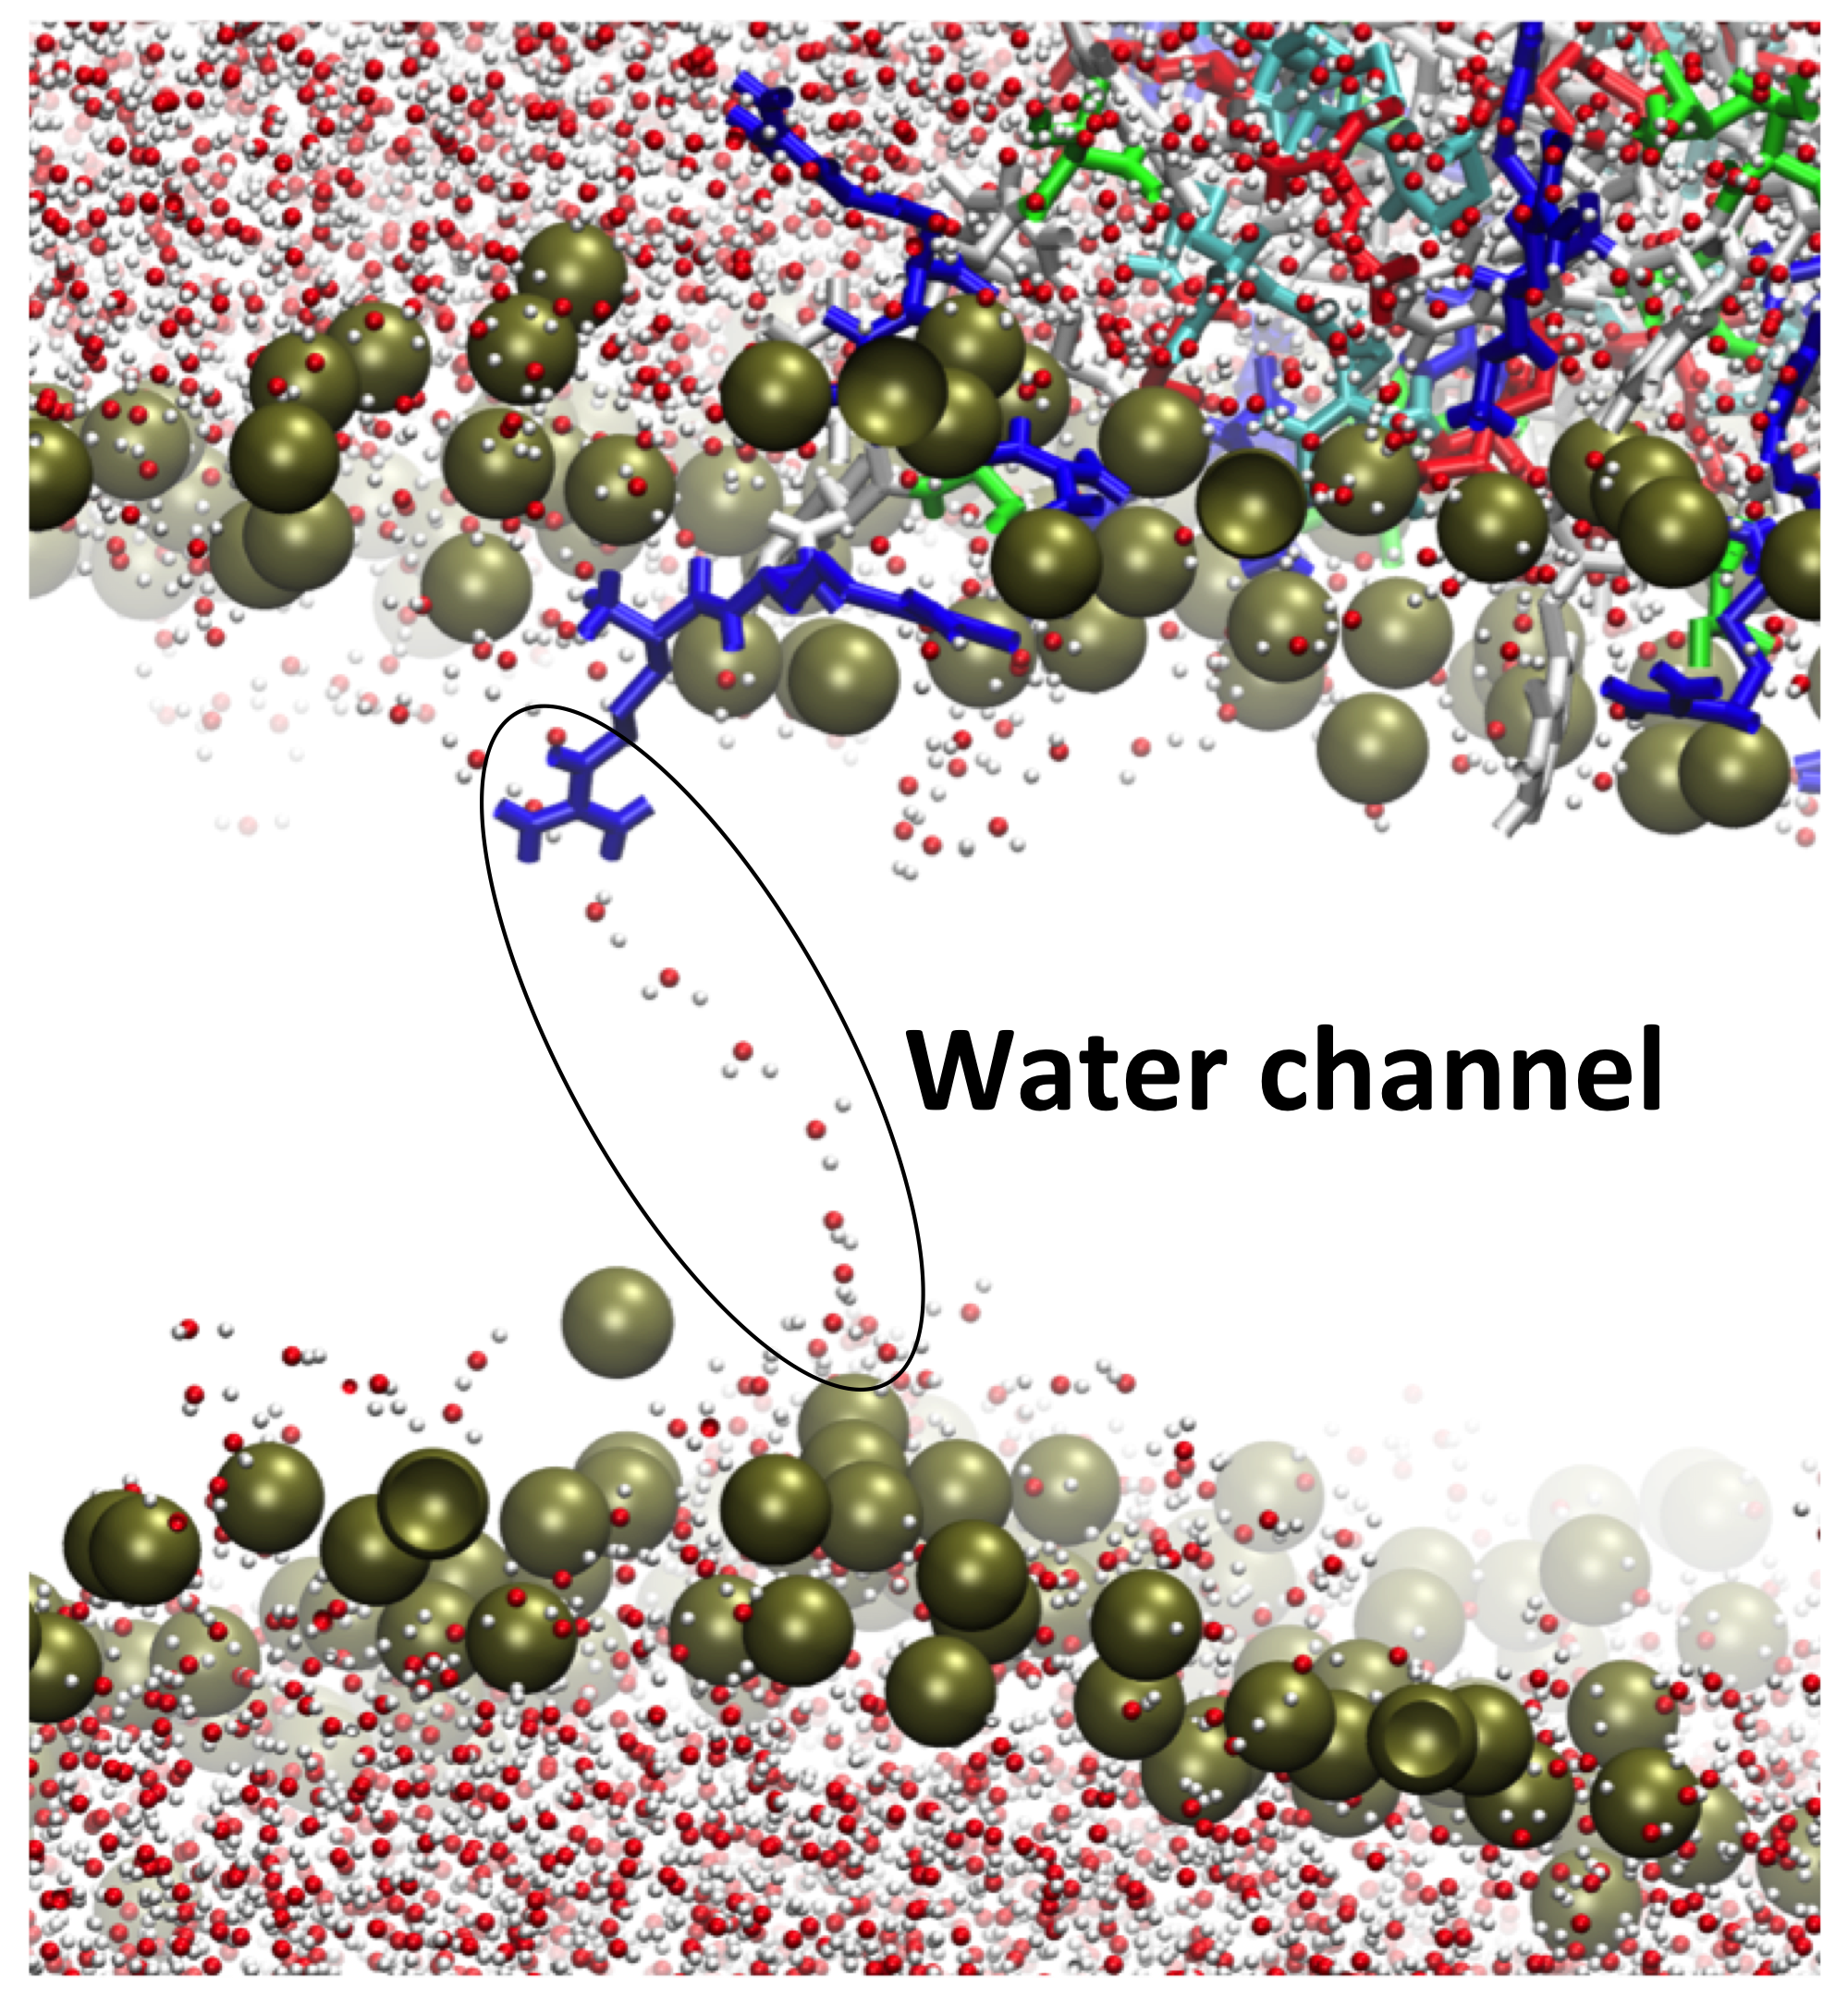
\includegraphics[width=40mm]{3results_capsule/pics/pore_arg.png}
\label{fig:pore_pics_3}}
\end{minipage}
\caption[Snapshot from relevant membrane-peptide simulations]{(a) Membrane deformation due to an electric field applied to the membrane (512 lipids, E = -130 mV/nm). (b) Pore formation due to the action of the peptide. (c) Pore precursor due to Arginine insertion and water penetration. [VMD software \citet{HUMP96}]}
\label{fig:pore_pics}
\end{figure}

The field was increased of 20 mV/nm every 200 ns (or 10 mV/nm when approaching the poration threshold), showing that the critical value of 130 mV/nm triggered poration in presence of the peptide. The initial value of 20 mV/nm was chosen as it is an approximation of the physiologic value of the transmembrane potential.
%
This was confirmed by three replicas run with a 130 mV/nm field from the initial unperturbed membrane configuration (poration after 20 ns, 75 ns and 71 ns respectively).
%
Similarly, on the 740 lipids patch in presence of capzip the same field induced membrane disruption after 60 ns, 50 ns and 70 ns respectively (Figure \ref{fig:pore_pics_2}).

As a control, a pure 512 lipids bacterial membrane is simulated under the same conditions, in three replicates: in the 600 ns runs, we observed the appearance of curved regions (Figure \ref{fig:pore_pics_1}) but no poration.
%
The appearance of a curvature made necessary to compute the area per lipid taking this into account, as explained in Section \ref{sec:analysis}. The three replicas gave values of 0.520 nm$^2$, 0.514 nm$^2$ and 0.550 nm$^2$. Their discrepancy is due to the different level of curvature the membrane adopts during the run (as they can change at a fast pace, the values given above were computed over the last 10 ns only).
%
It is observed that once a deformation appears it can be quickly enhanced by the electric field. Small casual variations in its initial onset can bring to very different shapes of the membrane.

The electroporation threshold for the membrane alone was set at the higher value of 140 mV/nm: out of three simulations run with such value of the electric field, two resulted in disruption at 150 ns and 154 ns, while the third presented a curved but still intact membrane after 200 ns.
%
This shows that the effect of the peptide shift the threshold by a small amount in absolute terms, but its action is clearly accelerating the disruption process.

The simulations with high electric field performed on the 512 lipids patch resulted all in curved geometry before the poration event (independently from the presence of the peptide). However this does not happen with the large patch, for which the poration was always initiated from a flat membrane conformation (Figure \ref{fig:pore_pics_2}).
%
To rule out once more the hypothesis that the difference is due to the force field used (54A7 versus 54A8), we run an additional control simulation of the 512 lipids patch with the 54A8 force field and the electric field set at the electroporation threshold of 140 mV/nm. The patch developed a curved shape similar to the outcome from the corresponding 54A7 simulations. The membrane was not electroporated in the 200 ns run, as was observed in one out of the three replicas of the 54A7 simulations.
%
The ApL values of these two simulations (512 lipids, 140 mV/nm, no peptide) differing only for the force field (54A7 or 54A8) are quite similar: 0.554 versus 0.556 nm$^2$, which were computed taking into account the curvature.
%
However, from the previous electroporation simulations it emerges that there is a high variability in ApL computed from highly curved configurations, so that the consistency of the two values might be fortuitous.
%
Once more, this analysis proves that the size of the patch has a large influence in the outcome of the simulations.

Regardless the shape that the membrane assumes before disruption, the peptide speeds up the collapse mechanism. This is due to the charged Arginine residues which insert into the membrane core interacting with the negatively charged phosphate of the lipids, and promote the penetration of water molecule (Figure \ref{fig:pore_pics_3}).
%
Indeed, out of the hydrogen bonds between Arginine and lipids listed in Table \ref{table:hb_pr_lip}, the vast majority involves the oxigen of the ester group of the lipids, as shown in Table \ref{table:hb_ester}.

\begin{figure}[t!]
\centering
 \def\arraystretch{1.6}
\begin{tabular}{l|ccc|ccc}
\hline
& \multicolumn{3}{c|}{\textbf{E = 0 mV/nm}} & \multicolumn{3}{c}{\textbf{E = 20 mV/nm}} \\
\hline
& Total & Pho & CO$_n$ & Total & Pho & CO$_n$ \\ 
\hline
DLPC & 20 & 6 & 14 & 18 & 10 & 8 \\
DLPG &12 & 3 & 9 & 16 & 5 & 10 \\
\hline
 \end{tabular}
\captionof{table}[Hydrogen bonds between Arg and selected lipid moieties]{Number of the hydrogen bonds between Arginine residues and lipids, existing for more than 50\% of the time, in simulations of the 740 lipid bacterial patch with the peptide and electric field equal to zero or 20 mV/nm. Total number is displayed and the ones occurring with the Phosphate (Pho) moiety of the lipids or one of the ester groups (CO$_n$).}
\label{table:hb_ester}
\end{figure}

Additionally, the peptide enhances the invagination of the membrane and this, together with the Arginine insertion, allows pore formation at a value of the electric field lower than the one necessary for electroporation.

This findings, together with the previous results, suggests that the decrease in membrane fluidity (measured by the reduction of the diffusion coefficient), regardless the membrane compactness (measured by the area per lipid), is a proxy for poration as it makes the lipids less able to accommodate perturbations and to seal a forming water channel.


\subsection{Atomistic simulations of the mammalian model membrane} \label{sec:lip_atom_mamm}

After the investigation of a model bacterial membrane, we focussed on a mammalian one, modelled as a DLPC patch. Given the information accumulated in the previous investigation, we simulated directly a large patch (748 lipids), as we deemed this size more appropriate to run the subsequent simulations with the peptide. The force field employed is GROMOS 54A8.

The properties of the stand alone membrane are computed as before and compared with the experimental data. Indeed for mono-lipid membranes several experimental results are available. The computed ApL is 0.592(3) nm$^2$, while the experimental range at 303 K of temperature is 0.608-0.632 nm$^2$ (see Table 1 in \citet{Poger2016}). To motivate the discrepancies, two factors must be considered. First, these experiments are performed on a variety of lipid geometries, from vesicle to supported lipid bilayers (resting on a solid surface), justifying the broad range of values. Second, the membrane is simulated in presence of a 150 mM salt concentration, while the experiments do not adopt it. Several computational studies report a reduction of area per lipid when salt concentration is introduced \citep{Bockmann2003,Jarerattanachat2013,Reif2017}. This is consistent with the experimental evidence \citep{Pabst2007}, even though simulations are reported to overestimate this variation \citep{Reif2017}.

This hypothesis is supported by the results from a simulation of a 512 patch without salt, which gives ApL of 0.626(5) nm$^2$. This is 0.034 nm$^2$ larger than the run with 748 lipids and salt mentioned above, and compatible with the experimental values (see Table \ref{table:dlpc_apl} for a summary). We do not have a similar comparison for the 748 lipids membrane, but this trend of salt induced shrinking has been confirmed by simulations of various patches for which the salt concentration was the only difference (see SI Table --).
%
Therefore, we conclude that the effect of the salt concentration is the main responsible for the membrane shrinking we observe in the simulations run at 150 mM.

The ApL of the DLPC patch is larger than the one for the model bacterial membrane, likely due to the presence of DLPG which diminishes the repulsion between the positively charged Choline heads of DLPC. Somewhat counter intuitively, the lateral diffusion coefficient is significantly smaller (0.495(1) $\mu$m$^2$/s). This is confirmed by the values found for the 512 lipid DLPC patch without salt (see Figure 8 in Chapter \ref{chapter:lip_par}).
%
The motivation for this augmented mobility when DLPG is present is hard to establish [COMMENT?].

\begin{figure}[t!]
\centering
 \def\arraystretch{1.6}
\begin{tabular}{lllll}
\multicolumn{5}{c}{\textbf{Pure DLPC}} \\
\hline
& Lipids & Salt (mM) & ApL (nm$^2$) & D ($\mu$m$^2$/s) \\
\hline
\multirow{3}{*}{\rotatebox{90}{\textbf{Apo}}} & 748 & 150 & 0.592(3) & 0.673(1) \\
& 512$^a$ & 0 & 0.626(5) & 0.541(1) \\
\cline{2-5}
& Exp.$^b$ & 0 & 0.608-0.632 & 3 \\
\hline
\textbf{Peptide} & 748 & 150 & 0.592(4) & see Table \ref{table:dlpc_D_space} \\
\hline
 \end{tabular}
\captionof{table}[ApL and D of DLPC (atomistic simulations)]{Area per lipid and pure diffusion coefficient of DLPC (atomistic simulations). All simulations run with the GROMOS 54A8 force field. $^a$ Run with 1.4 nm cut off. $^b$ Experimental values. Area per lipid from Table 1 of \citet{Poger2016}, diffusion coefficients from \citet{Lindblom2009}.}
\label{table:dlpc_apl}
\end{figure}

The presence of the peptide does not affect the ApL of the DLPC patch, as it was observed for the bacterial counterpart (on the same size patch). Computing the diffusion centring the trajectory with respect to the peptide (Table \ref{table:dlpc_D_space}), we observe an increase in the diffusion coefficient with respect to the pure one displayed in Table \ref{table:dlpc_apl}, likely because of the movement of one leaflet with respect to the other. The lipids closer to the peptide are still slowed down as observed in the bacterial membrane, albeit they are more mobile in absolute terms.

Analysing the number of hydrogen bonds formed with the peptide, there are 590 bonds, of which 19 present more than 50\% of the time. Of them, 11 involves Arginine residues, which coordinate with ester groups in 6 cases, and with phosphate in 5 cases. This figures are smaller than the ones obtained for the bacterial membrane. In particular, the absence of the charged lipids makes the protein-membrane interaction less favourable.

\begin{figure}[t!]
\centering
 \def\arraystretch{1.7}
\begin{tabular}{ll|ll}
 \multicolumn{4}{c}{\textbf{Pure DLPC}} \\
 \hline
 & Region & Nr. & D ($\mu m^2/s$) \\
 \hline
\multirow{4}{*}{\rotatebox{90}{\textbf{Peptide}}} & $d<1$ & 100 & 0.495(3) \\
& $d<2$ & 180 & 0.584(3) \\
& $d<3$ & 323 & 0.603(5) \\
& $d>3$ & 412 & 0.993(5) \\
& All & 735 & 0.821(2) \\
 \hline
\multicolumn{2}{l|}{\textbf{Apo global}} & 748 & 0.673(1) \\
 \hline
 \end{tabular}
\captionof{table}[D coefficient in proximity of capzip (mammalian membrane, atomistic)]{Diffusion coefficients of lipids, computed centring the trajectory around the Protein COM, in a 740 lipids DLPC patch, simulated in presence of the pentagonal peptide subunit. Coefficient for apo simulation displayed for comparison. The values are computed for groups of lipids which, at the initial time, were within 1 nm, 2 nm, 3 nm from the peptide or further away. The values for the patch simulated without the peptide are reported as reference. Error from linear fit in parenthesis.}
\label{table:dlpc_D_space}
\end{figure}

On the DLPC patch, we did not perform the same extensive electroporation analysis carried on for the bacterial membrane. Instead, we simulated directly the threshold electric field value (130 mV/nm). 

However, for the DLPC patch this value is sufficient to cause poration both with and without peptide. Despite the absence of lipids with a net charge, which are expected to interact more strongly with the electric field, this membrane seems more sensitive to such external perturbation. We think this is due to larger ApL: indeed, being the lipids less packed, water penetration is easier. This, combined with the electric field, generate a water defect which promote pore formation.

Once the membrane start disrupting, the peptide detaches from the membrane, while it remained firmly attach to the bacterial one, following its deformations. This lower propensity for binding on the mammalian case will be proven also by coarse grain simulations.

In interpreting these results, it must be considered that the transmembrane potential of a mammal cell is lower than the one present in the bacterial membrane \citep{Yeaman2003,Wilson2011}, so that the conditions to which the peptide is exposed to are different in proximity of different cells. We do not pursue the investigation of the electroporation threshold for the DLPC patch, as we focus here only on the action of the peptide on it.

Finally, if the lower interaction with DLPC is consistent with the selectivity of capzip against bacterial membrane, it must be reconciled with the fact that capzip internalisation is observed on HeLa cells. This will be discussed more extensively in the next section, where the approach of a capsule to model membranes is investigate by coarse grain simulations. [COMMENT - DO DISCUSS]


\subsection{CG simulations of the buckyball on model membranes} \label{sec:results_lip_cg}

\paragraph{Standard MARTINI simulations} Coarse grain simulations allow to model the behaviour of the full capsule interacting with the membrane.
%
At first, simulations with the standard MARTINI model were run, due to their higher computational speed (the full system, comprising a 2880 lipids patch and the capsule, measures approximately 30 nm along each side of the simulation box).

Coarse grain simulations of the full buckyball on a DLPC:DLPG membrane (3:1 ratio) confirms the binding of the peptide on the latter, driven by charge-charge recognition: in both the replicas run, the peptide approaches the membrane after about 2 $\mu$s, remaining bound up to the 10 $\mu$s simulated.
%
Post-binding, the capsule diffuses on the membrane and produces an increasingly high curvature on it, in a process which tends to maximize the contact area (see Figure \ref{fig:pL6_vmd_2} and SI Movie --). No poration is observed, probably due to the force field characteristics which stabilise the structure of both the membrane and the peptide assembly. Additionally, longer time scales might be needed to observe poration. In the next paragraph, we will perform simulations with an additional electric field, in line with what done in the atomistic case, which speed up the process and allow to observe membrane disruption.

\begin{figure}[h!]
\centering
 \def\arraystretch{1.5}
\begin{tabular}{ll|ll|ll}
\multicolumn{6}{c}{\textbf{Mixed membrane}} \\
 \hline
 && \multicolumn{2}{c|}{MARTINI} & \multicolumn{2}{c}{Polar MARTINI} \\
 \hline
 \multicolumn{2}{l|}{E (mV/nm)} & DLPC & DLPG & DLPC & DLPG \\\hline
 \multirow{2}{*}{0} & Apo
	& 74.28(1) & 73.34(2) & ?? & ?? \\
 				& Prot. & 70.51(1) & 62.59(2) & 65.82(6) & 68.94(9) \\
\multirow{2}{*}{20} & Apo & NA & NA & 74.64(5) & 73.67(2) \\
 	& Prot. & NA & NA & 70.29(7) & 61.54(10) \\ 
 \multirow{2}{*}{40} & Apo & NA & NA & 70.312(4) & 70.45(6) \\
					& Prot. & NA & NA & \multicolumn{2}{l}{Poration} \\
 \hline
\end{tabular}
\captionof{table}[Lipid diffusion coefficient for coarse grain bacterial membranes]{Analysis of lipid diffusion in a coarse grain simulation of the buckyball binding to a model bacterial membrane (DLPC:DLPG 3:1). Diffusion is computed removing the centre of mass movement of the bilayer for simulations without the capsule, and of the protein for simulations where the peptide is bound to the membrane.}
\label{table:martini_diff_bact}

\begin{tabular}{l|ll}
\multicolumn{3}{c}{\textbf{DLPC membrane}} \\
 \hline
 E (mV/nm) & MARTINI & Polar MARTINI \\
 \hline
 E = 0		  & 81.07(3) & 70.50(2) \\
 E = 20 & NA & 75.28(6) \\
 E = 40 & NA & 77.88(4) \\
 \hline
\end{tabular}
\captionof{table}[Lipid diffusion coefficient for coarse grain mammalian membranes]{Analysis of lipid diffusion in a coarse grain simulations of a mammalian model membrane (DLPC) in presence of the capsule. Details on computation of diffusion as in Table \ref{table:martini_diff_bact}.}
\label{table:martini_diff_dlpc}
\end{figure}
%
When analysing the diffusion coefficient, the values obtained before the binding have been computed removing the movement of the membrane centre of mass, while the ones after by centring the trajectory around the capsule.
%
The lipids diffusion is decreased after the binding, by 5\% for DLPC and by 15\% for DLPG (Table \ref{table:martini_diff_bact}). Moreover, as DLPG is negatively charged, it is recruited around the peptide and remains bound to it, so that some molecule of this specie diffuse much slower than the surrounding lipids. Indeed the average number of lipids which are within 2 nm of distance from the capsule after its binding to the membrane is 167(10) for DLPC and 131(7) for DLPG. Considering that DLPG constitutes only 25\% of the membrane, this proportion indicated that negatively charged lipids migrate toward the peptide.
%
Additionally, each of this molecule is closer the peptide than the average DLPC molecule: computing the RDF of the phosphate beads (PO4) of DLPC and DLPG around the protein, a much stronger signal comes from DLPG beads rather than DLPC ones (Figure \ref{fig:PO4_RDF}).
%
\begin{figure}[t!]
\centering\includegraphics[width=0.6\linewidth]{3results_capsule/pics/RDF_PO4_around_Prot.png} 
\caption[Proximity of lipids phosphate to bound capsule]{RDF of phosphate bead (named PO4 in both MARTINI models) of DLPC and DLPG around the Protein.}
\label{fig:PO4_RDF}
\end{figure}

To conclude the investigation performed with standard MARTINI, we simulated the capsule together with a pure DLPC membrane. The capsule does not bind to it in the 10 $\mu$s simulated: it comes close to it multiple times, with an average distance of 3 nm and a minimum of 1 nm, but never gets in contact with the lipids. This, together with what already observed in the atomistic simulations, suggest once more that the interaction with non charged lipids is not favourable.

\paragraph{Polar MARTINI simulations} 
The Polar MARTINI simulations focussed on \emph{in silico} experiments with an external electric field, to set a parallel with the analogous atomistic ones.

We took the membrane patches equilibrated with the standard MARTINI and employed them without performing a further equilibration. The structure of the capsule was taken from a Polar MARTINI run. As performed in the atomistic case, together with the simulations with the capsule, we run control simulations of the membrane only with the external field of the values chosen, to exclude the possibility of electroporation.

Regarding simulations with the capsule, we first run a simulation without electric field, to test the interaction between the two components with the new parametrisation. The binding happens much faster than what observed in the standard MARTINI simulations, and the membrane starts to be deformed by the capsule already after 100 ns. However, we did not observe poration on the timescale of the simulation (500 ns). A longer simulation might allow to observe membrane disruption but, as mentioned before, we preferred to focus on the action of the electric field. As such, we simulated the binding under the action of a 20 mV/nm electric field. The curvature of the membrane is slightly more pronounced than in the case without field, and the membrane seems more rigid (Figure \ref{fig:martini_stMem} and SI Movie --), but without any disruption. From the final configuration of this run we doubled the electric field, which was sufficient to observe poration within 200 ns.

\begin{figure}[t!]
\centering\includegraphics[width=0.95\linewidth]{3results_capsule/pics/picmartiniPW.png} 
\caption[MARTINI simulations of capsule on membrane]{[REDO]}
\label{fig:martini_stMem}
\end{figure}

As in membrane simulations the pressure coupling is performed semi isotropically, once a pore is formed, the box undergoes a large and unphysical deformation if the pore keeps expanding. To obviate to that, we took a frame at the early staged of pore formation and continue the run, with the same electric field, with isotropic pressure coupling. This allowed to observe how the capsule penetrated the membrane causing a whole in it: the lipids do not seal around the capsule, allowing for passage of water and ions. This is consistent with what found in the atomistic simulations. Moreover, in the passage, the capsule deforms and partially opens.
%
Being the field still present, the capsule is pushed through the simulation box, and keeps spanning its range.

As a control, the same simulations were run with a DLPC membrane: for none of the values of the electric field tested (0, 20 and 40 mV/nm) the capsule bound to the membrane.

The diffusion coefficient was measured also for simulations with Polar MARTINI. For the DLPC membrane, the increase of the electric field...



DISCUSS
why small field (only 20/40)


ADDSelf assembly, new model lammps what to do, D amino acids

\section{Outlook}


\section{Rest}
%
%
%
%

%
%
%%\paragraph{Membrane binding mechanism}
%A coarse-grain simulation of the full buckyball on a DLPC:DLPG membrane (3:1 ratio) confirms the binding of the peptide on the latter, driven from charge-charge recognition: in both the replicas run, the peptide approaches the membrane after about 2 $\mu$s, remaining bound up to the 10 $\mu$s simulated (the binding happens on opposite leaflets of the membrane, proving that it is not biased by the initial configuration).
%%
%Post-binding, the capsule diffuses on the membrane and produces an increasingly high curvature on it, in a process which tends to maximize the contact area (see SI Movie --). No poration is observed, probably due to the force field characteristics which stabilise the structure of both the membrane and the peptide assembly or the short time scale simulated.
%%
%The lipids diffusion coefficient is decreased after the binding, by 9\% for DLPC and by 15\% for DLPG (see SI Table \ref{table:SI_martini_diff} and SI Figure \ref{fig:SI_martini_lipids_bound}).
%Moreover, as DLPG is negatively charged, it is recruited around the peptide and remain bound to it, diffusing much slower than the surrounding lipids.
%
%A control simulations with a pure DLPC membrane shows no binding of the peptide: the distance of the icosahedron from the membrane is on average 3 nm and never smaller than 1 nm. This does not exclude a binding on longer time scales, but hints at the fact that, not being driven by the opposite charge recognition, the peptide-membrane interaction is weaker and less likely to happen.
%
%
%\section{Conclusions}
%
%In the present work, we propose a model structure for the three dimensional arrangement of a novel antimicrobial peptide, testing the stability of the proposed model by means of Molecular Dynamic simulations. Furthermore, we investigated the details of its antimicrobial activity simulating its interaction with a model bacterial membrane.
%
%The simulations performed on the peptide assembly and on its subunits highlighted the preferred conformations: a staggered $\beta$-sheet favouring Tryptophan interactions and the stacking of $\beta$-sheets pairs to confer stability to the assembly by screening the hydrophobic residues and to grant rigidity.
%%
%The structure of the single molecule suggests an ordered geometry of the supra molecular assembly to optimise the number of interaction between peptides, however the simulations proved that the molecule is not rigid enough to form a virus-like cage, while a dynamical equilibrium is enforced in which the components have the freedom to fluctuate around the equilibrium position.
%
%These findings are important to direct future design of similar molecules, as the rigidity and mechanics of the capsule structure are crucial to tune its function as carrier and its interactions with the host cells.
%
%Regarding the interaction with a bacterial cell instead, simulations make clear that the peptide has a complex effect on the membrane, prior to its disruption: its presence enhance its rigidity, making it prone to disruption upon local triggers such as Arginine insertion. This support the necessity of a self-assembling antimicrobial peptide, as the higher the local concentration of antimicrobial molecules, the more the deviation from the base line membrane properties, which favours an early disruption.
%
%Overall, the work shows how Molecular Dynamics simulations give precious information on the atomistic-level mechanisms underlying mesoscopic processes: despite the limitations of the technique prevent sometimes a quantitative interpretation of the simulations result, MD proves the qualitative aspect of various processes and can be effectively used to compare different systems and identify the local characteristics which lead to diversified behaviours. This will suggest the design of new experiment to specifically tackle aspects based on emerged via simulations and thus finally prove the MD findings.
% 

%
%\clearpage
%\section{SI miscellaneous}
%
%\begin{figure}[h]
%\centering
%\includegraphics[width=0.85\textwidth]{pics/rep1_sch_BM.png}
%\caption{\textbf{[BETTER QUALITY]} Contacts with persistence greater than 50\% during a backmapped atomistic, between C$_\alpha$s (left column), between side chains (middle column) and mixed C$_\alpha$-side chain (right column).}
%\label{fig:SI_BTI_contacts}
%\end{figure}
%
%
%
%\clearpage
%
%
%\begin{figure}[h]
%\centering
% \def\arraystretch{1.5}
%\begin{tabular}{l|rr}
% \multicolumn{3}{l}{\textbf{MARTINI simulations - capsule on bacterial membrane}} \\
% \hline
% & \textbf{DLPC} & \textbf{DLPG} \\
% \hline
% D pre-binding ($\mu \text{m}^2$/s) & 298.81(3) & 294.14(7) \\
% D post-binding ($\mu \text{m}^2$/s) & 273.11(3) & 249.57(6) \\
% N$_{<\,2\,nm} \ ^a$ & 167(12) & 131(7) \\
% N$_{bound} \ ^b$& 197 & 115 \\
%\end{tabular}
%\captionof{table}{Analysis of lipid diffusion in a coarse-grain simulation of the buckyball binding to a model bacterial membrane (DLPC:DLPG 3:1). Data for Replica 1, binding time 2.14 $\mu$s. Protein lateral diffusion after binding to the membrane 16.50(2) $\mu$m$^2$/s. $^a \, $Number of lipids within 2 nm distance from the buckyball in the last 5 $\mu$s of simulations. $^b \, $In a simplistic model in which the dumping of lipid lateral diffusion coefficient is due to some lipids bound to the buckyball, and thus they diffuse at its pace, while the other are free to move as before, it is valid the following equation: $D_{post} = D_{pre} \cdot (N_{lipid} - N_{bound}) + D_{protein} \cdot N_{bound}$.}
%\label{table:SI_martini_diff}
%\end{figure}



\clearpage
\section{Additional material}




\begin{figure}[h]%[p!]
\centering
 \def\arraystretch{1.6}
\begin{tabular}{ll|l|l}
\hline
 \multicolumn{2}{l|}{\textbf{No peptide}} & Bacterial & Mamm. \\
 \hline
 \multirow{2}{*}{E = 0} & 512 & \emph{54A7} (1) & \emph{54A7} no salt (1) \\
 & 740 & \emph{54A8} (1) & \emph{54A8} (1R) \\
 \hline
 \multirow{2}{*}{E = 130} & 512 & \emph{54A7} (3) & -- \\
 & 740 & -- & \emph{54A8} (1) \\
 \hline
 \multicolumn{4}{l}{+ Bact/512/E-140: \emph{54A8} (1R)} \\
 \hline
 \multicolumn{2}{l|}{\textbf{Peptide}} & Bacterial & Mamm. \\
 \hline
 \multirow{2}{*}{E = 0} & 512 & \emph{54A7} (1) & -- \\
 & 740 & \emph{54A8} (1) & \emph{54A8} (1R) \\
 \hline
 \multirow{2}{*}{E = 130} & 512 & \emph{54A7} (3) & -- \\
 & 740 & \emph{54A8} (3) & \emph{54A8} (3) \\
 \hline
 \end{tabular}
\captionof{table}[Force fields employed for atomistic runs of model membranes]{Table of the simulations run for different systems. Electric field expressed in mV/nm. For each cell, the syntax reports: Nr. of lipids \emph{Force field} (Nr. of replicas).}
\label{table:membrane_simulations_force_field}
\end{figure}


\section{Supplementary material} \label{sec:ch3_SI}

We include here additional material, Figures and Tables referenced in the chapter which can help the reader in interpreting the results.


\subsection{On the long range electrostatic cut off}
In a few paragraphs of this chapter we compare the simulations run here with the ones from the parametrisation work in the next chapter. As the reader will see, these are run on 512 lipids patches, with a simulation set up very similar to the one employed here.

However, the long range electrostatic are treated with a Reaction Field scheme and cut off radius of 1.4 nm. This choice was performed for consistency with previous parametrisation work.
%
Instead, the simulations run in the present chapter are run either with the Reaction Field and a cut off of 1.2 nm (512 lipids patches) or with a Particle Mesh Ewald treatment, and the same cut off (740 lipids patches).

Although briefly mentioned in the body of the chapter, we want to reiterate that these discrepancies might affect the simulations, but in measure smaller than the peptide or the electric field, which effect we want to assess.

Indeed, extensive literature on the effects of long range electrostatic treatment suggests that electrostatics have an influence on the ApL up to 0.010-0.015 nm$^2$ only. This is confirmed for the change in the cut off treatment (single or double) \citep{Silva2018,Reisser2017}, and the switch from PME to RF [\citet{Poger2012}; Table 1 in Chapter \ref{chapter:lip_par}].
%
The only conditions which severely affects the ApL seems the complete neglect of the long range electrostatic, choosing a plain cut off scheme \citep{Patra2003}.

Regarding the different cut off values, we did not find previous work testing the difference. However, given that we apply a long range correction, the cut off simply discriminated which positions are treated in the exact way and which instead through the long range approximation of choice. As these approximations seem consistent among them and robust, we foresee that a small shift in the cut off length does not have a high impact on the simulation outcome.


\subsection{Supplementary figures}
\begin{figure}[h!]
\centering
\includegraphics[width=0.6\linewidth]{3results_capsule/pics/bb_contacts.png}
\caption[Final configuration of a pentagonal subunit simulation]{Final configuration from a 100 ns simulation of the pentagonal subunit in solution. Bonds and cartoon representation, coloured by name. [VMD software \citet{HUMP96}]}
\label{fig:penta_results_SI}
\end{figure}

\subsection{Supplementary tables}
\begin{figure}[h!]
\centering
 \def\arraystretch{1.6}
\begin{tabular}{lccccc}
 \hline
 \multicolumn{6}{c}{\textbf{Pure membranes and electroporation simulations}} \\
  \hline
  & Lipids & $\,$FF$\,$ & $\,$Time (ns)$\,$ & E (mV/nm) & Rep. \\
 \hline
 \multirow{8}{*}{\rotatebox{90}{Bacterial}} & 512 & GR (54A7) & 400 & 0, 70, 120 & 1 \\
 & 512 & GR (54A7) & 600 & 130 & 3 \\
 & 512 & GR (54A7) & 150$^{P}$, 154$^{P}$, 200 & 140 & 3 \\
 & 512 & GR (54A8) & 200 & 140 & 1 \\
 & 740 & GR (54A8) & 400 (350) & 0 & 1 \\
 & 740 & GR (54A8) & 400 & 20 & 1 \\
 %\hline
 & 720 & MA & 1000 & 0 & 1 \\
 & 2880 & MA\_P & 500 & 20, 40 & 1 \\
 \hline
 \multirow{4}{*}{\rotatebox{90}{Mamm.}} & 748 & GR (54A8) & 400 & 0 & 1 \\
 & 748 & GR (54A8) & 20$^{P}$, 28$^{P}$, 39$^{P}$ & 130 & 3 \\
 & 722 & MA & 1000 & 0 & 1 \\
 & 2888 & MA\_P & 500 & 20, 40 & 1 \\
 \hline
\end{tabular}
\captionof{table}[Control atomistic simulations of pure membranes]{Table of control simulations of membranes complexes. All run at 150 mM concentration of NaCl. Force fields (FF): GR = united atom GROMOS, MA = coarse-grain MARTINI, MA\_P = coarse-grain MARTINI with polar water. Superscript P refers to the rupture of the membrane (poration).}
\label{table:SI_membrane}
\end{figure}
